% Load the kaobook class
\documentclass[
	fontsize=10pt, % Base font size
	twoside=false, % Use different layouts for even and odd pages (in particular, if twoside=true, the margin column will be always on the outside)
	%open=any, % If twoside=true, uncomment this to force new chapters to start on any page, not only on right (odd) pages
	secnumdepth=1, % How deep to number headings. Defaults to 1 (sections)
]{kaobook}

% Choose the language
\usepackage[english]{babel} % Load characters and hyphenation
\usepackage[english=american]{csquotes}	% English quotes

% Load packages for testing
\usepackage{blindtext}
%\usepackage{showframe} % Uncomment to show boxes around the text area, margin, header and footer
%\usepackage{showlabels} % Uncomment to output the content of \label commands to the document where they are used

% Load the bibliography package
\usepackage{kaobiblio}
\addbibresource{intro-pubinv.bib} % Bibliography file

% Load mathematical packages for theorems and related environments
\usepackage{kaotheorems}

% Load the package for hyperreferences
\usepackage{kaorefs}


\graphicspath{{images/}{./}} % Paths where images are looked for

\makeindex[columns=3, title=Alphabetical Index, intoc] % Make LaTeX produce the files required to compile the index


\begin{document}

%----------------------------------------------------------------------------------------
%	BOOK INFORMATION
%----------------------------------------------------------------------------------------

\titlehead{Public Invention}
\title[Public Invention]{Public Invention}
\author[RLR]{Robert L. Read}
\date{\today}
\publishers{Public Invention, a US public charity}

%----------------------------------------------------------------------------------------

\frontmatter % Denotes the start of the pre-document content, uses roman numerals

%----------------------------------------------------------------------------------------
%	COPYRIGHT PAGE
%----------------------------------------------------------------------------------------

\makeatletter
\uppertitleback{\@titlehead} % Header

\lowertitleback{
	\textbf{Disclaimer} \\
	You can edit this page to suit your needs. For instance, here we have a no copyright statement, a colophon and some other information. This page is based on the corresponding page of Ken Arroyo Ohori's thesis, with minimal changes.

	\medskip

	\textbf{Copyright 2022, Robert L. Read} \\
%%	\cczero\

	\medskip

	\textbf{Colophon} \\
	This document was typeset with the help of \href{https://sourceforge.net/projects/koma-script/}{\KOMAScript} and \href{https://www.latex-project.org/}{\LaTeX} using the \href{https://github.com/fmarotta/kaobook/}{kaobook} class.

	\medskip

	\textbf{Publisher} \\
	This book has not yet been printed. \@publishers
}
\makeatother

%----------------------------------------------------------------------------------------
%	DEDICATION
%----------------------------------------------------------------------------------------

\dedication{
  If you want to build a ship, don’t drum up the men to gather wood, divide the work, and give orders. Instead, teach them to yearn for the vast and endless sea.\\
  \flushright -- Antoine de Saint-Exupéry
  \\
  The chances of your success are zero, but the importance is infinite; therefore, I support you.\\
  \flushright -- Sir W. Lawrence Bragg

}

%----------------------------------------------------------------------------------------
%	OUTPUT TITLE PAGE AND PREVIOUS
%----------------------------------------------------------------------------------------

% Note that \maketitle outputs the pages before here
\maketitle

%----------------------------------------------------------------------------------------
%	PREFACE
%----------------------------------------------------------------------------------------

\chapter*{Preface}

This is a draft work whose purpose is explain and promote Public Invention as a
movement and philosophy.
This work will likely be published electronically by Public Invention (the organization),
but we will also seek a print-publisher who is willing to keep the work open access.

-- Robert L. Read

%----------------------------------------------------------------------------------------
%	TABLE OF CONTENTS & LIST OF FIGURES/TABLES
%----------------------------------------------------------------------------------------

\begingroup % Local scope for the following commands

% Define the style for the TOC, LOF, and LOT
%\setstretch{1} % Uncomment to modify line spacing in the ToC
%\hypersetup{linkcolor=blue} % Uncomment to set the colour of links in the ToC
\setlength{\textheight}{230\vscale} % Manually adjust the height of the ToC pages

% Turn on compatibility mode for the etoc package
\etocstandarddisplaystyle % "toc display" as if etoc was not loaded
\etocstandardlines % "toc lines as if etoc was not loaded

\tableofcontents % Output the table of contents

\listoffigures % Output the list of figures

% Comment both of the following lines to have the LOF and the LOT on different pages
\let\cleardoublepage\bigskip
\let\clearpage\bigskip

\listoftables % Output the list of tables

\endgroup

%----------------------------------------------------------------------------------------
%	MAIN BODY
%----------------------------------------------------------------------------------------

\mainmatter % Denotes the start of the main document content, resets page numbering and uses arabic numbers
\setchapterstyle{kao} % Choose the default chapter heading style

\pagelayout{wide} % No margins
\addpart{Why Be a Public Inventor}
\pagelayout{margin} % Restore margins

\chapter{“Invent in the public, for the Public.”}


Benjamin Franklin (1705-1790) did not patent the Franklin stove because
he believed it to be too useful an invention to legally encumber.
He has been
called ``The First American''\cite{Brands2000}, but I think of him as the
first Public Inventor.
If you read the autobiography of Nikola Tesla (1856-1943)
``My Inventions''\cite{Tesla1982},
you discover a devout public servant
(in a non-denominational sense), who certainly wanted to make
money but whose deepest motivation was to see human progress.
R. Buckminster Fuller (1895-1983) wrote extensively on the act of invention
as a moral act: nerve gas is bad, vaccines are good\cite{Fuller1981}.
Richard Stallman (1953-) articulated the principles of free software
and in so doing indirectly increased the wealth and well-being
of the planet tremendsouly\cite{Stallman2002free}.
This book is my attempt to extend and promote the work of
those inventors to create a stronger movement which we could
call public invention.\marginnote{We have created a non-profit, also called Public Invention, but will try to keep the very important movement distinct from the relatively unimportant legal entitity.}

\nocite{laurel2001}
\nocite{jonassalk}

Invention advances human progress spectacularly.
Politicians mostly ignore it.
Human history is largely a story of technological
advance careening foward from the stone age with
an inexorably building speed,
perhaps to a frighetning climax.
Those who believe it will end in a dark and terrible
destruction are not fools;
but that fate is not certain.
We as a planet can choose instead to build a bright future
in which humanity explores the universe together in peace.
This will happen only if we understand technology as the
powerful moral force that it is.

For the last 100 years, technological advance has been driven
by two engines: profit and academic research.
The modern emphasis of Universities on patenting research
and the governmental practice of subsidizing research which
is monopolized by for-profit firms has blurred the distinction between the two.
Nations have long recognized the value of technology for
competiting with other nations via
war or mercantilism. Public invention hopes to be a movement
that does not replace for-profit research and academic research,
but becomes a third engine. The motto of Public Invention
is ``Invent in the public, for the Public.''

\begin{marginfigure}[-5.5cm]
    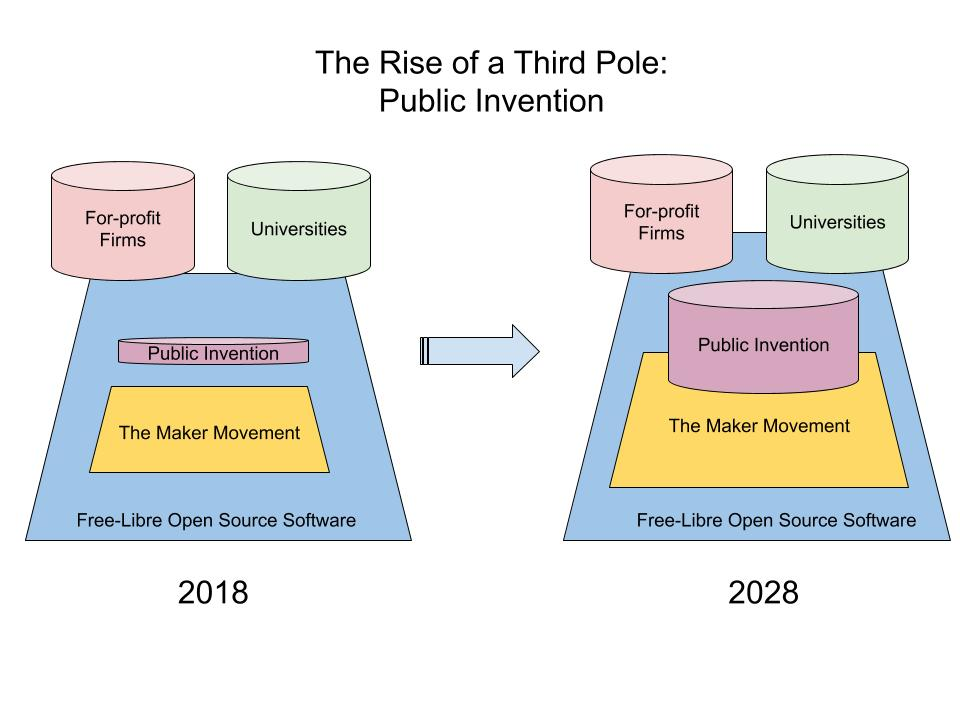
\includegraphics{figures/The_Rise_of_Public_Invention.jpg}
  \caption{The Rise of Public Invention as a Third Pole of Progress}
  \labfig{rise}
\end{marginfigure}

This means the public inventor does not seek monopolies in
the form of patents or other intellectual property but
gives an invention freely to the whole world without prejudice.
Anyone is free to use the invention, including for the purpose
of making a profit, but nobody is given
exclusive rights to it.

Buckminster Fuller made a clear distinction between what he
called ``killingry'', or weapons, and ``livingry''--that
which increase the good in the world.
The public inventor
must not build weapons.
This is impossible
to do perfectly;
even a pillow can be used as murder weapon.
Nonetheless,
technologists are not relieved of the moral duty to invent
good things instead of bad things just because it is
intellectually difficult to make the distinction.
The public inventor accepts this burden and does the best they can.

Benjamin Franklin said, ``We must, indeed, all hang together or,
most assuredly, we shall all hang separately.''
His wit was poignant because he meant the American revolutionary
leaders would indeed have swung from a British rope for treason
if the Revolutionary war had been lost.
But in 2022 his words ring true globally. Buckminster Fuller
believed that humanity would either destroy itself or
have a bright, Star Trek-like future---there is no
middle ground.
We cannot continue to muddle along
taking weak action on global warming.
The COVID-19 pandemic has shown that we are all connected
in a most intimate way, whether we like it or not.
A disease incubated in my body may kill you, and vice versa.
Therefore the public inventor must at some level seek
the wealth and health of the whole world.
Narrow national chauvinism is no longer a useful or profitable
behavior.

We could define public invention simply as invention in the
public interest.
In that sense, it is closely related to humanitarian engineering.
Humantarian engineering requires a great deal of problem-solving,
innovation, and ingenuity.
The distinction is that ``invention''
means something truly novel which has never existed before.
Public  invention values the truly novel, whereas
humanitarian engineering values the truly useful.

In the future, it will be common place for people to move freely
between
the three engines: for-profit firms, academic research,
and public invention.
Public invention will not replace the other two engines,
but augment them.
Inventing in the public, for the Public is a moral act, but it is not a moral duty.
Some people will be called to be public inventors some of the time.

\chapter{The Joy of Public Invention}

It is easier to be a motivated public inventor
if one sees oneself as a minor character in a great story,
the greatest story that we can know, the story of human progress.\marginnote{``You can be the captain, and I will draw the chart..." -- Rush, Closer to the Heart.}
It does not particularly matter if you believe this progress
is positive or negative, though Steven Pinker is has argued overwhelmingly it
is astoundingly positive. \cite{Pinker2019}
You may see the story originating in
Babylonia, Egypt, Athens, Jerusalem, the Chin dynasty, the
Enlightenment, or the American Revolution as you see fit.
The more history you know, the better, of course.
Being part of a great story gives your actions meaning.
Your life will not be measured out in coffee spoons
if you see yourself as part of a great story.\marginnote{TODO: Cite the LoveSong of J. Alfred Prufrock}

Much science fiction is dystopian and dark, but almost all
places humanity in the arc of some great story,
in which the characters are agents.
This is not as common in fantasy, but it is true of the
greatest fantasy.
Certainly, the Marvel Cinematic Universe, the Lord of the Rings,
Star Wars, Dune, the Space Trilogy of C.S. Lewis,
and the Chronicles of Narnia all accomplish this.
Distressingly, the idea of the arc of human progress is
less present in political statements\marginnote{I dare not say political discourse, which disappeared in America in 1994.}
than it was in my youth.\marginnote{As of this writing, a war is being executed not to move the arc forward, but to restore it backwards in time.}
Without a sense of where we have been and where we are going,
politics misses the point, and becomes mere tribal bickering.\marginnote{Richard Nixon spoke of population growth and control.
  Whether you agree or disagree, and no matter the messenger, it was a long-term vision.}

Public invention takes the inherent joy of invention and doubles
it with the joy of helping others.
Making something truly new is a roller coaster ride
of emotions.
The inventor is frought with doubts.
Is the invention even possible?
Has someone done this earlier?
Am I too stupid to accomplish this?
Often a new idea creates innumerable frustrations.
The expensive equipment breaks at a critical momemnt.
There may be collaborators,
but there are no experts to turn to, because by definition
the invention has never been made before.
Despite all of the doubts and frustrations, or
perhaps because of them, the eventual progress, if it
comes, is an intense joy.

Comic books and movies have taken a grain of truth
and mythologized it out of proportion to create the trope
of the lone inventor.
Most invention is done by teams.
Math, is, in the end, always social, even if each baby step is solitary.
The joy of collaboration is part of the attraction
of being a public inventor.

Each of us is unique and has unique gifts to bring
to the table.
In a sense this is true in any part of life,
but it is a especially true in the act of invention.
Each of us has a different voice, even if we sing
the same song.
However, by definition, invention is making something
not just new in the sense of a variation of something
old, however unique, but new in the sense of breaking new
ground.
An invention is not yet another hybrid rose, it is a new kind of flower.
Even mediocre inventors such as myself are essential and necessary.
The mediocre work makes the great work easier.

Some people have an invention inside them that has to get out.
The seed of an idea planted in childhood may mature in the unconscious
until the time is right for it emerge.
Sometimes this is because of a persons great love of something.
We have all seen people enchanting by flying or
infatuated with light.
Some people can spend years entranced by a math problem.
The inventions may be useful, but unprofitable.
Some may even be potentially harmful. Certainly many persons,
including myself, are fascinated by projecting things at
high velocity, such as in guns, rockets, bows,
catapults, or water guns.
So long as the invention is not designed to harm,
the invention should be allowed to be born, if not practiced.
The line between invention and art is sometimes blurred.
The public inventor should support whimsical inventions
when a person has a strong desire to make it.

The public inventor should not make fakes or toys.
That is, the public inventor should not make an object
whose value is that it is a miniature mockery of some
other object or like some other object which has intrinsic value.
Making a model of a beautiful airplane or ship is valuable
and fun, but it is not invention.
Making a fake starship is creative, but not invention.

However, the desire to make something new even if the
utility of the invention is hard to define should be
respected. This may be because it is artful, or may
have nothing to do with art, and its value may lie
in some other dimension.
Often, an invention that wants to be made that has
no clear purpose is a forerunner of something else
which cannot be conceived until the first invention
is reified and can be held in hand.

To me, public invention is really about love---love of humanity,
of beauty, of the planet, of math, and of my fellow-inventors.
For some of us, the joys of learning, collaboration, invention,
and helping the world melded together in public invention
is the greatest joy we can imagine.
At the end of my life my proudest acheivement will be my children,
and my second greatest sense of joy will come from the
inventions I have given the world, however small they may be.


\section{Myths and Tropes}

Myths motivate us.

Tropes and sub-myths shape our thinking.
The real psychological import of the fantasy worlds of the DC and Marvel universes cannot be escaped.
The sub-myth of the loner genius inventor as exemplified by Bruce Wayne, Lex Luthor, and Tony Stark
can both motivate us and lead us astray.
This book can be considered an elaboration of the lesson that Peter Parker, Spiderman, learned
in his origin story: ``With great power comes great resposibility.''\marginnote{Jesus said the same thing much earlier. (Matthew 25:14–30)}
We all have power, and if you can be a public inventor, you have great power. If you have great power, you have great responsibility.

The fictional inventors are surely inspirational at one level.
It makes a good and simple story for the slightly anti-social or sociopathic genius to come up with things more or less on their own.
The reality is that invention in isolation is not very effective.

If we move from pure fantasy to the merely legendary, there is no doubt that
some important inventions have been the work of nearly solitary minds.
Isaac Newton was not very amaible and by modern standards was highly secretive.
His impact would have been much greater if he had published properly rather than keeping his work secret.
He is among the greatest of scientists for creating the theory of gravity
all on his own and co-rediscovering calculus with Leibnitz\marginnote{It seems that Archimedes should be given the credit for the fundamental insight of the calculus, the infinitesimal change, although it was lost for two millenia with his death.}
Einstein also worked alone is 1905, the ``annus mirabilis'', in which he produced four ground-breaking papers.
Tesla created the AC motor in isolation. Well and good.

Yet we must not be fooled into thinking this is the only or even the dominant way in which humanity advances knowledge.
Thomas Edison was not the freakish genius that Nikola Tesla was, but invented more, generally with teamwork, for a while even with Tesla.
Marie and Pierre Curie discovered radium together and Marie Curie ran an effective laboratory after her husband's death, leading to her second Nobel prize.
Today, it is not uncommon for dozens of persons to be named in a Nobel prize announcement, because science has become social.
Many feats of engineering which are not technically individual inventions nonetheless are groundbreaking enough to
be called ``modern wonders of the world''.
Examples would be the Hubble space telescope, the Apollo moon launch, the Tesla electric vehicle, the modern 3D printer, and automatic genome sequencers.
Yet these engineering feats are creating by very large teams, and can be created no other way.

I recommend that we seek new fictional characters for inspiration or to emulate. Hermione Granger is a fine example, because like Bruce Wayne and Tony Stark,
she has no special abilities.[TODO: Add Citation]
Nevertheless she excels by working hard and doing her homework. Like Harry and Ron, her greatest strength is in the end her
teamwork and friendships.

Sadly, fantasy tends to be more exciting than reality.
Reality is long nights in a lab and delaying fun now to do your homework to have a greater fun later.
The cold reality is that we are not all geniuses and that even geniuses struggle.
But, the public inventor must toil, but need not be lonely---we are all in this together.

\section{The Interstellar Expansion Myth}

Science fiction is the literature of ideas; it would not be worth the name if it were not astoundingly diverse.
Nonetheless, the Myth of interstellar travel dominates science fiction.
I use the word ``Myth'' here not to mean a falsehood, but to mean a foundational story that gives meaning.
Many science fiction stories suggest a basic conjecture, which we could call the Interstellar Conjecture[TODO: This is not typesetting correctly]:

\blockquote[Interstellar Conjecture]{
  There exist other planets around other stars, and it is possible and desirable for humanity to travel to them and live there.
}

Our telescopes and technology have now identified more than 5000 exoplanets[TODO: Add citation], so this
conjecture is unlikely to fail due to a lack of planets. How many of them may
be in any sense habitable after how ever much terraforming or habitat building
remains a mystery, but if only one in a thousand it suitable, then it may
be in theory possible.
It is my fondest hope that we will someday explore those planets together in peace.

Technological improvement is inexorable. If technology can find a holdfast, however small,
it can generally climb upward. In the case of travel between stars however, we have no
such foothold today and can conceive of none. The closest idea we have is the ``generation ship'',
the dubious idea of building a ship that would take so long in travel that real generations of
human beings would be born and die in that small space before reaching any interstellar
destination.

Interplanetary travel within the solar system is coming in decades.
Interstellar travel is a myth today,
and may or may not become real in a century or a millenium. It may not be possible, ever.

It may not even be desirable. C.S. Lewis, in his Space Trilogy[TODO: add Citation], puts the believe that
it is desirable into the mouth of one of the great villains.
Mores specifically,
Dr. Westin asserts that humanity should not just travel to other stars but to dominate them;
to colonize them,
if possible, and if they have inhabitants, to wipe them out of subjugate them as seems most convenient
to ensure the eternal expansion of the human race.
Lewis found this idea diabolical.
He was attacking no straw man. In the science fiction of the first half the 20th century, this
idea was indeed quite common. I'm ashamed to say I bought into it as a boy.
The idea that we could visit other inhabitedd planets and bring them some sort of gift (as I would wish)
or even simply not disturb them or ruin them seems dubious to me.
I am nervous disagreeing with Lewis;
but I suppose we could mature as a species from our current mewling infancy so that perhaps someday[TODO: Cite La Infana Rasa]
we need not be a plague on the galaxy.

Put putting that question aside, the Interstellear Conjecture seems pernicious to me in another way.
It suggest that we need not be custodians of our solar system and Earth. It suggests that Earth
is disposable. For the next 500 years this is hellish folly. There is nowhere else to go home to.
We must either heal the Earth or fail.

Obscuring this fact with false hopes is not useful.
A reader may think such a false hope is harmless because it is irrelevant.
This book argues that that is not true; humanity needs public inventors, and they need to be working
on the most valuable inventions.
We need to create livingy, not killingry.
If we put their hopes in the false Interstellar Conjecture, we will be less likely to invent
things that heal the Earth.

\chapter{Why it makes more sense than in the past}

Participation in public invention makes more sense with
each passing decade.
Although we suffer from inequity, in raw terms the world
is more abundant than ever before.
Commodities are cheaper.
Fewer people live in poverty.
The number of people who are financially able to take
a few months out of the work force to work on a public invention
project without compensation is higher than ever.
Philanthropists are more generous than ever before.
The number of people who make a substantial income
essentially through patronage and tipping is probably
higher than ever before.
In a world of abundance, the need to make a profit
or to work relentlessly at a career should
diminish.

In America today, housing in large cities
and formal education are exceptions
to the general trend of things becoming cheaper and easier to obtain.
Participating in public invention is a powerful way to
obtain two things provided by a formal education:
learning and reputation.

There are specific technical reasons certain kinds of
public invention are far more accessible than ever before.
In the first place, the internet has made many tutorials
and how-to documents available almost for free, from
how to use a soldering iron to very sophisticated academic
papers.
Secondly, the free software movement has made an ocean
of high quality software available.
Although it takes effort, almost any computing task can
now be accomplished without paying a cent for software.
It remains the case that some of the best scientific tools
do not yet have free-gratis alternatives of similar quality,
but the trend is incontrovertible: the cost of computing
is getting cheaper.
I'm writing and typesetting this book right now
using mostly free software tools.
This same software generally also makes it cheaper to
build new software.
Usually, software that it free
as in free-pizza is free as in free-speech---meaning that
anyone has the freedom to use it as a starting point for making
something new.
Software has limitations, but it is extraordinarily versatile.
It is the most general-purpose of all technologies. The fact
that it is free is a fundamental enabler of public invention,
because capital attracted based on expectations of profits is
not needed.

Hardware is more expensive, but has gotten dramatically
more accessible at a low price. 3D printers that cost USD\$300
can now make astounding object that could scarcely exist 30
years ago. Similarly, it is now possible to design printed
circuit boards on free software and have them fabricated
and very low costs, usually in about two weeks.
This capability augments the old-fashioned but still
useful soldering iron as a means of making sturdy circuits.
Of course the reduction in the price of computers, which
includes single-chip micro-contollers used in electronic
embedded systems, is legendary.

Although I am weak on bio-hacking, I believe the same
expansion of capability at reasonable cost has occurred in
the word of biology, microbiology, and genetics.
Even optics, in the form of microscopy and telescopy,
has seen major improvements.

Batteries and solar power have enabled deployment of
electronics portably and to remote off-the-grid locations.
Significant improvements in cameras, sonar, and other
sensors have also increased the sophistication available
at low cost.

(Create Matrix/Infographic of relative acceleration in fields.)

Although hardware cost remain a relative imepdiment\marginnote{see Chapter \ref{chp:material} for Public Invention's policy},
the combination of cheap hardware, free software, and
cheap connectivity enables easy innovation and invention.
Sharing and publication of inventions is also
ever easier.

\section{Makers into Public Inventors}

Makers know the fundamental human joy of making.
The Maker movement supports creativity, skill building,
art, humor, and practical function.
Makers today, thanks in large part to Make magazine[TODO: add citation]
and Maker Faires, have thousands of fascinating
projects to prove from.
Their projects are very diverse, from fiber arts to
3D printing to microelectronics to amateur science.
Perhaps millions of people consider themselves Makers.
If the public invention movement could co-opt even three per cent
of the energy of the maker movement, the benefit to the world would
be astounding.

An invention by defintion has to be something
which has never been made before.
Making is not easy; it takes practice, problem solving, creativity,
and ingenuity, but usually not invention.
There is a natural path from making to
public inventing which some makers will follow.
This book is an attempt to create
for the public invention movement
a culture as strong and supportive as
Maker culture is today.

It is also an appeal to Makers to band together and
take on more ambitious projects by growing into
actions of humanitarian engineering and finally public invention
or open science.
Millions of Makers know the joy of making.
Clothes, tools, and machines are the extended phenotypes of human beings,
as necessary to us as a tortoise shell is to it.
They know the satisfaction of creating something beautiful with
their hands.
They know the relief of finally getting a computer program to work
properly.
They get to see their friends admire the sweater they knitted,
or the robot they built.
This joy is both personal and social.
The exercise of the making mind and the athlete's muscles is
the same sort of satisfaction.
It is an intrinsic part of what it means to be human.
A part of this joy is overcoming the difficulty of learning
a new skill.

In general, you can eventually make something with enough
patience. I normally have to try several times before my
craft work starts to become satisfactory, but in general
the knowledege of how to do it is freely shared.
One has to practice, but one need not innovate.
In the end you are making something that has been made
before, perhaps thousands of times.
The fact that it can be made by hands only a little
steadier and mores skillful than one's own is not in doubt.

The risk of utter failure is much higher when researching
an invention.
Many ideas, perhaps most ideas, will simply never work.
It is entirely possible to spend several years on something
that in the end amounts to nothing which you can demonstrate.
You may still have gained a lot, but
it may not be anything of physical beauty, utility, financial value,
or prestige.

Nonetheless if just a small fraction of the creative energy
and effort put into Making for fun could be channeled into
public invention, humanity would make much greater progress.

\chapter{The millifuller}

\begin{marginfigure}
  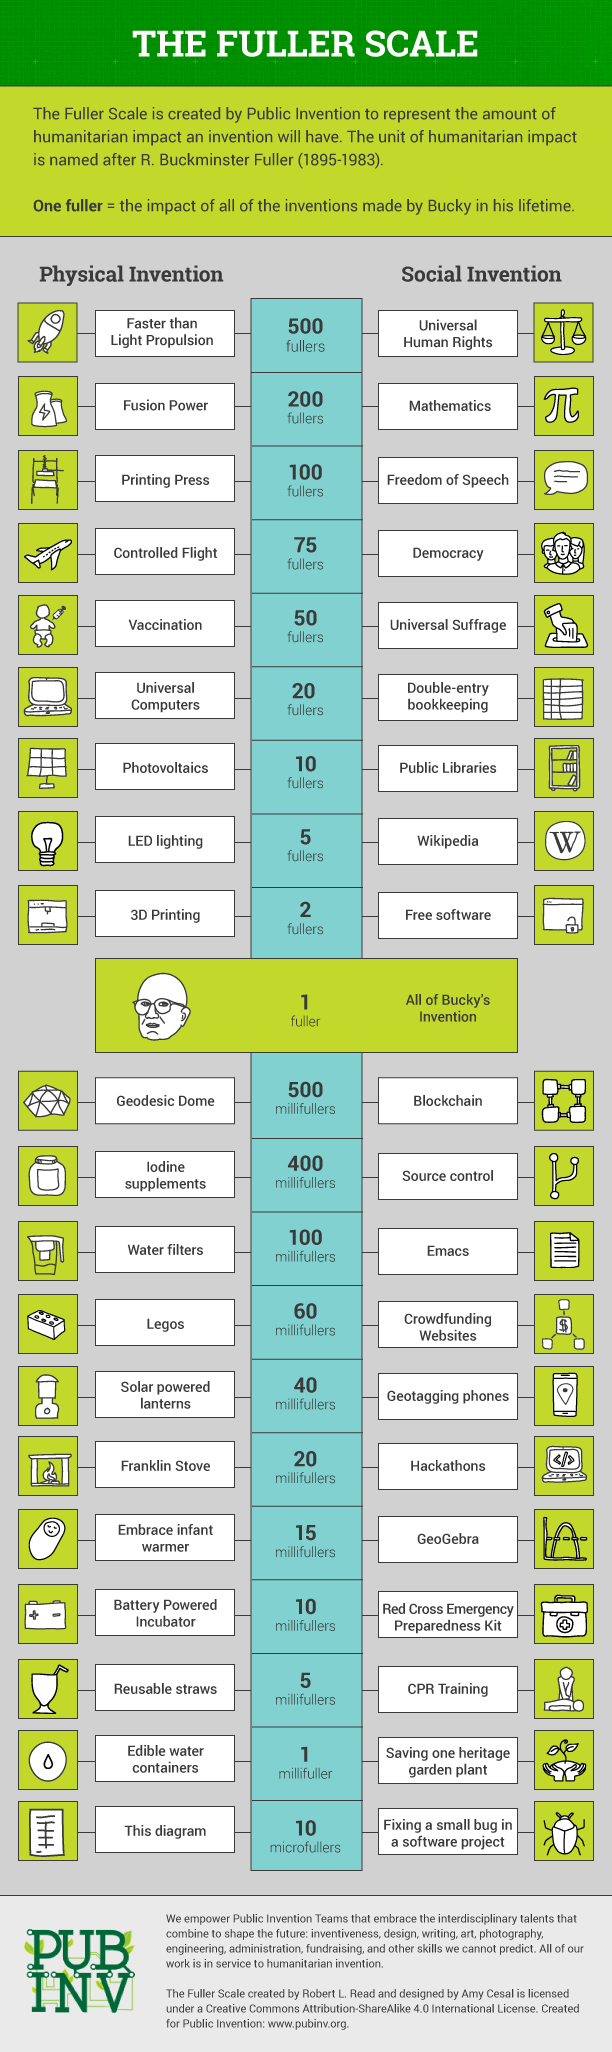
\includegraphics{figures/FullerScale.png}
  \caption{The Fuller Scale of Humanitarian Invention Value}
  \labfig{fullerscale}
\end{marginfigure}

Science is about truth; engineering is about compromise.

Public inventors do both, but perhaps more engineering than
science.

Our goal is to have a large positive impact on many people; but time
and money are always in short supply.  How, then, to compromise on
which projects to prioritize?

In order to be able to prioritize two
projects that may compete for attention, it helps to be able to measure
humanitarian impact in some way.
To do this, we have created “The
Fuller Scale“. The “fuller” is a new unit of humanitarian impact,
inspired by Buckminster Fuller, the great American champion of
invention as a moral good. It is by definition the impact of all of
the inventions of his long life.

It is, of course, subjective; the best things in life are.

A team of inventors does not need to agree perfectly to usefully
quantify impact. I hope in the future Public Inventors and other will
have conversations like:

“Well, I agree your robot technology is a useful search-and-rescue
idea. If it is worth 20 millifullers, then surely detecting
contaminated drinking water, which kills 270,000 children every year,
is worth at least 40 millifullers!”

“Yes, but free software for transparent accounting is equally
important, and easier to develop!”

“Well, it may be easier, but it can’t be more important—let’s call it
30 millifullers.”

“Okay. But if we can do it in one year, that about 3.5 millifullers a
month of value added to the world; that robot thing is going to take
years. I doubt you will get more than 1 millifuller a month doing
that!”

And so on.

Note that in our diagram, we have social inventions, such as Universal
Suffrage, on the right, and physical inventions on the left. The world
is broad, and there is room for improvement everywhere.

Like everything we do at Public Invention, The Fuller Scale and its
diagram is Free-libre open source content.
In this case it is licensed
under the Creative Commons Attribution-ShareAlike 4.0 International
(CC BY-SA 4.0) license, which means you are free to share it, extend
it, and even change it, so long as your retain a pointer back to
Public Invention and its inventors (Robert L. Read and Amy Cesal, the
graphic artist, in this case.) It is in a GitHub repo that you can
fork. Please share.

\chapter{Imagining what it will be like}

\section{The Near Future}

\begin{figure}
  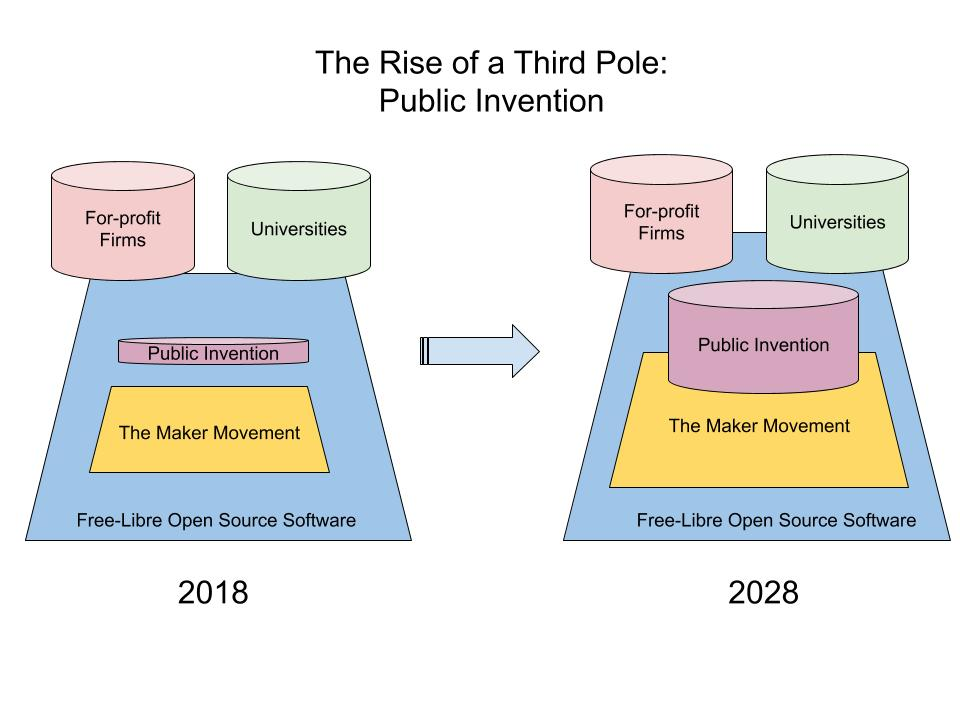
\includegraphics{figures/The_Rise_of_Public_Invention.jpg}
  \caption{The Rise of Public Invention as a Third Pole of Progress}
  \labfig{rise}
\end{figure}

With your kind permission, let me take you on an
imaginatvie journey into the near future of the next 20 years.

There will be three engines of economic growth:
for-profit research, universities, and public invention.
People will flow smoothly between these three.
A young researcher might start volunteering for public invention while
looking for a good job, move to that job, then go back to school
as a student or a lecturer,
then back to work, then back to public invention.
Profit is one of many tools of motivation, competing with
the status and recognition of universities and public invention.

When a person has a three-month hiatus between jobs or a
high school teacher has a summer off, it is easy for them to find
a public invention project to work on, because there is a
well-catalogued and maintained list of projects to which they can  match
their talents and desires.
Everyone kind of knowledge worker can contribute, because
there is high demand for technical writers, photographers,
graphic artists, managers, quality assurance experts, etc.
Skilled makers can contribute PCB designs or hand-soldered boards.
Woodworkers, metalworkers, 3D print makers, and other craftspersons
can find a list of needs and quickly produce something contributing
to a project.

Universities remain exclusive, and people compete to get in as
both students and faculty.
Public Invention remains inclusive, and people compete to
be recognized for their contribution. Gratitude begins
to hold its own againt vanity.

The landscape of projects is driven by human curiosity and
altruism. Finding needs to be addressed by public invention
by adding to the list of potential projects is a recognized
contribution.

Everyone who wants a mentor can find a mentor if they
show they are willing
to do the work to be worthy of mentoring.

Material costs of projects, but not labor, is financed by
charities that serve an evaluative function on the projects,
guaranteeing donors that their gifts have high impact.

When a person has an invention idea, they have a choice.
They can attempt to monopolize it and have a small chance at
a large profit, or they can donate it public invention and
have certainty of a small recognition.

The current near-monopoly on sophisticated medical devices held by
large corporations has been eroded by open-source designs
created by public inventor in response to health crises that
began with the COVID-19 pandemic 20 years earlier.
A much greater competition by medium sized firms has led to
greater innovation. In the low and middle income countries,
medical care still lags the wealthiest countries, but is
clearly catching up rapidly.
Open access to medical data and training materials is a
part of this process. Colleges, universities, and clinics
have open-source versions of ventilators, imaging devices,
anesthesia machines, lowering the cost of training.

A growing public commons of free and open designs
across the entire spectrum of possible inventions
is mined by corporations and both large and small to provide
new devices at reduced research costs.

Universities have mostly abandoned patenting their research
and now by default release all of their work in open-access journals
and under open-source licenses. Universities compete with each
other not only the quantity and quality of their research, but
on their openness and humanitarian impact.

Philanthropists and funding foundations provide perhaps three
dollars out of every ten to public invention projects.

People go to parties and say things like ``I'm a public inventor''
and everyone knows what they mean.
Although, just as today, with open source projects, a majority
of public invention projects uknown and obscure, but
everyone once in a while at a party someone will say in hushed tones,
``See that person with the ombre dyed hair? They were the
leader of the oxygen concentrator team in 2025.''

\section{The Far Future}

In 2122, the first class of Solar Fleet Academy is matriculated.
Money is still in use for luxuries and to fund world wonders,
such as the first generation ship, but is largely irrelevant
for basic food, clothing, and shelter.

There are now 50 billion people on Earth and 5000 off-Earth
and inside the asteroid belt. The carbon footprint of human
society is now less than it was in 1945. Global warming
remains a problem but CO2 levels are declining.

The constant improvement of energy storage, renewable energy sources, fission and fusion
has made energy cheap and non-polluting.

The oceans are clean and productive. The by-catch has been
eliminated; only the fish that are actually eaten are taken.
The reefs that were lost to global warming are being carefully
reconstructed.
Whole new ocean biomes are being created: floating reefs
that increase the diversity of the ocean directly.
The oceans produce abundant small fish and custaceans; large fish are luxury
eaten a few times a year.

The forests are half-way to fully recovering.
People gather that was never worth gathering before in forests
with the help of tree-climbing spider monkey robots.
Many parts
of the earth are both wilder and more economically productive than
they were previously.
Mature trees are carefully selected, cut and sawn into timber
in place.
The boards carried out by gentle walking robots that leave footprints
no bigger than bears.
Forests are many times more productive of wildlife, mushrooms, and timber
than ever before.

The restored bison herds of the North American plains provide 1/10th of the meat
for the entire planet.
Hunting is carefully regulated but game is abundant.

Agriculture has been transformed into small scale gardening.
Robots and
artificial intelligence allow hyper-efficient yields from small
spaces.

Although the population has increased, the total land
used for agriculture has gone down.
Basic food is cheap and produced by a few large factory farms.
Mmany people are engaged in producing
very high-quality foodstuffs locally based on genetically engineered
plants tailored to micro-biomes.
Professional farmers make a living on plots as small as 1000 square meters.

Biohacking has reached new levels, driven by necessity and
pleasure.
A student in England just engineered an English pea plant
whose pods open and spill out 100 multi-colored peas like unzipping
a purse of pearls.
There are tomatoes for 413 distinct micro-climates.
Luxury furniture is now grown in place as a single tree
controlled by hormones and rigid frames
matched exactly to body contours.

Forms of art unthought of in 2022 are flourishing.
Most people know and care very little about public invention,
and are engaged in their own pursuits.

Travel is inexpensive. High-speed trains
flow beneath the bicycle paths that have been built across the oceans.
Educational resources are cheap, but personal teachers are in high demand.
Infectious diseases are something taught about in history classes.

A highly organized and efficient rescue corps address natural disasters,
whether local or global.
Nations no longer fight wars of territorial control.

The public inventors live in a wonderland of possibilities.
Each public inventor has access to an enormous library of
scientific thought and access to design tools unimagined in 2022.
The average high school student can create designs of
complexity unimaginable in 2022, and can order them
produced at a reasonable cost.
Fabrication of integrated electromechanical devices is
done at the touch of a button locally.
The range of materials available for crafting includes
diamond, titanium alloys, fibers of unimaginable strength,
and intelligent polymorphic materials are approaching flubber.

The role of public invention in the success of the world is
debated. The Inevitablists claim that success was alway inevitable.
The Constructivists claim that success was constucted based on
specific policy decisions, individuals, and organizations.
The public inventors just keep inventing.

\chapter{The Stoic Point of View}

The ancient Stoics taught a practical philosophy that is only
tangentially related to the common meaning of the English word ``stoic''.
In terms of metaphysics, they believed that we should live in
accordance with nature, and it is natural for humans to use the reason
gifted to them by the Gods, if they exist---the Stoics were not
universally either deistic or non-deistic.

The first principle of Stoicism
is to distinguish between that which you can control, and that which
is outside your control.  You can control only your own actions, and,
with practice, your thoughts. The thougts dye the soul.  You cannot
control what others think of you.  The praise of others is the clacking
of tongues.  Being in the ``inner ring''---the faculty club, or being
invited to the exclusive conference, or to Lady Boodle's dinner party,
is not worth a fig.
\marginnote{
  I believe that in all men’s lives at certain periods, and in many
  men’s lives at all periods between infancy and extreme old age, one
  of the most dominant elements is the desire to be inside the local
  Ring and the terror of being left outside.
\url{https://www.lewissociety.org/innerring/}}
Alexander the Great and his mule driver are both gone to the same place,
and nobody remembers much about Alexander except his name.

The Stoics saw each of us as a part of a great community, each a
tiny part of a tiny society in a large Universe.
What is good for Society is good for the Individual.\marginnote{This is similar to the idea that we are all cells in the Body of Christ.}

Stocism is a great aid to the public inventor,
because it armors one against disaspointment and frustration.
It sees little value in accumulating enormous wealth.
It asserts that reason is a gift, perhaps a divine gift,
to be used for the betterment of all.
Even the spiders and bees have their useful occupation.
Some of us are born to farm, to entertain, to build, and
some of us are born to be public inventors.

The Stoics believed that reason was a gift to humans from the Logos.
The Logos might be interpreted as divine reason, or directly
as God or the Gods.
The ability to reason allows us to be more than beasts
and to participate, at least partially, in the divine.
They meant this in several senses.
Reason keeps us from being inebriated
all day, although as brutes we may find this pleasant.
Reason makes us behave civilly towards our
fellows, although it is, on the surface, to our advantage
to steal from them.

Today, classes in philosophy are really the study
of the history of philosophy, rather than philosophy itself.
To them philosophy, literally the love of wisdom,
meant the study of how to live well.
Because we are gifted beyond other animals in having
reason, it is our duty use our reason to learn how to live
well.
To the Stoics, this spanned personal hygiene,
how to behave at dinner parties, how to be a citizen
of your city-state, and even how to be a citizen of the world.

In the classical period of Stoicism, Universities had
not been invented, and their was no model for either
the private inventor or the public inventor of physical
inventions.
A small number of philosophers may have procured a
living by inventing the constructs of philosophy, but
even then only indirectly.
However, I assert that in the modern world, Stoics
should agree that being an inventor is a worthy profession
just like being a farmer, a policeman, or a teacher.

The Stoics cultivate {\em preferred indifference.}
They were not opposed to wealth.
It is better to be rich than to be poor,
but one can be good and happy while poor.
But they would agree with modern psychologial research
that once a basic level of material wealth is obtained,
additional wealth is not particularly valuable.
If you have enough, whether you have more than enough
or just enough should not make you unhappy in either case.
One may prefer to have more than enough, but one should
not be distraught at having less than enough.

Marcus Aurelius was strongly communitarian.
He wrote that what is good for the body politic (by which
he meant both the Roman empire and all humanity) is good
for the individual.
In general the Stoics did not have a strong sense of
an immortal soul.
They believed death was a transmutation of the elements,
and that is was natural for a person to be born, participate
in humanity, and then die.
The physical body was given by the mother, and
then by food, until eventually it was transformed back into
the elements from which it came.
The mind or soul came seemingly from nowhere and went
seemingly to nowhere.
This should not be counted a loss
or a sadness, as nothing has been removed which was not
given as a temporary gift in the first place.
Humans, just like the plants, the beasts of the fields,
and even the insects, had their job to do.
In ancient Rome there was less freedom to choose
one's occupation than there is today.
To the Stoic, being good consisted in doing the assigned job
well, whether you were an ox, a slave, a soldier, or an emperor.

The public inventor uses reason on behalf of the
universal community without much regard for their own
profit.

It seems to me the Stocis would have approved of public invention.
[TODO: Add citations for all of this section.]

\chapter{The Christian Point of View}

\marginnote{I am a devout Unitarian-Universalist. Most Christians would not call me a Christian,
  though I have been highly influenced by Christianity.}

We must admit from the outset that Jesus was not
an electrical engineer.
He never touched a soldering iron, though a soldier's iron touched Him.
There are limits to what the words attributed to Christ and his followers
can directly mean for public invention.

This is the Great Commandment:
\blockquote{
... and one of them, a lawyer, asked him a question to test
him. "Teacher, which commandment in the law is the greatest?" He said
to him, "'You shall love the Lord your God with all your heart, and
with all your soul, and with all your mind.' This is the greatest and
first commandment. And a second is like it: 'You shall love your
neighbor as yourself.' On these two commandments hang all the law and
the prophets."
}\marginnote{Matthew 22:35-40}

The great innovation of Jesus was Love.
The Stoics before Him and many other philosophies extolled ethics
and kind, civil behavior.
A Stoic would share their bread with you, out of duty.
A Christian would share their bread with you, out of both love and duty.
The love/duty duality is reflected in the great Christian debate
of the importance of faith (the Augustian view) and good works (the Pelegian view).
C.S. Lewis and most mature thinkers view them as intertwined.\marginnote{But not me---I belive good works matter far more than faith, a view which is officially heretical to many Christians, and related to the heresy of Pelegianism.}

God is the Creator, the Prime Mover, the First Maker.
Dare I say God is the prime Inventor?
To love God with all our heart, our soul, and especially
with all our mind, means to love and study His creation, creatures, and work.
I therefore consider all sciences, not least mathematics, to be branches of theology.

The second part of the Great Commandment is to love you neighbor
as yourself.
Surely this means that I must share my inventions and knowledge
with my neighbor just as I share my bread.
The Great Commandment requires sharing, and sharing requires
free-libre open source licenses.
Free software and free hardware is therefore a Christian commandment.
Some us are surely
meant to be public inventors and to love our neighbors
by providing them open-source ventilators and machines to provide clean drinking water.

The parable of the talents (Matthew 25:14–30)
is apt. A ``talent'' was gallon jar of silver coins, but
the parable was metaphoric to begin with, and we can
by happy coincidence use the normal meaning of the English word
``talent'' here.
Talents must not be buried!
Surely those who have the inclination to study math and physics
have a talent, because assuredly not everyone is so inclined.
There is support for this idea from St. Paul as well:
\blockquote{
  Whatever your hand finds to do, do with all your heart.}
(Ecclesiastes 9:10)

In Ephesians, Paul establishes the metaphor of the ``body of Christ'',
which parallels the Stoic view of the community of humanity.
\blockquote{
  11 So Christ himself gave the apostles, the prophets, the evangelists, the pastors and teachers,
  12 to equip his people for works of service, so that the body of Christ may be built up
  13 until we all reach unity in the faith and in the knowledge of the Son of God and become mature, attaining to the whole measure of the fullness of Christ.

  14 Then we will no longer be infants, tossed back and forth by the waves, and blown here and there by every wind of teaching and by the cunning and craftiness of people in their deceitful scheming.
  15 Instead, speaking the truth in love, we will grow to become in every respect the mature body of him who is the head, that is, Christ.
  16 From him the whole body, joined and held together by every supporting ligament, grows and builds itself up in love, as each part does its work.
}
(Ephesians 4:11-16)

This same idea, that each of us has a precious originality,
has the modern catchphrase: Don't forget to be awesome.[TODO: fine this reference]
``Awesome'' in this case means to be your true self.
I personally believe this is the meaning of ``salt of the earth'' saying:
\blockquote{
  13 “You are the salt of the earth. But if the salt loses its saltiness, how can it be made salty again? It is no longer good for anything, except to be thrown out and trampled underfoot.
}(Matthew 5:13)
This idea is echoed by C.S. Lewis:
\blockquote{
  “Even in literature and art, no man who bothers about originality will ever be original: whereas if you simply try to tell the truth
  (without caring twopence how often it has been told before) you will, nine times out of ten, become original without ever having noticed it.”
}(Mere Christianity)
The Public Inventor must choose projects as the inner light guides them.[TODO: Cite Quakerism here.]
The choice of what to work on cannot be reduced to an algorithm.
The work of invention should be a thrilling, wild adventure.
There will be drudgery but the work itself must remain loved
by the inventor.

Jesus was many things, but by tradiditon his profession
before his ministry began is translated into English as ``carpenter'', but
David Bentley Hart has more recently translated the Greek ``tectos'' as
``builder''\cite{hart2017new}. Jesus was a builder. It is not a play on words to say
He was a Maker.
According to the gospel of John and the Athanasian Creed which enshrines
the Trinity, Jesus was the Word\marginnote{The Greek in John uses ``Logos''. The logos is of exceptional importance to the Stoics, where it can be translated as
  ``reason'' or ``nature'' or ``divine reason''.}and the Word with God at the beginning,
so was also the Maker.

Christians are called to be ``Christ-like''. This is not usually interpreted to mean,
``be a maker if you are given a God-inclination to make'', but I see this as
a Biblically supported view.
C. S. Lewis would have us be ``little Christs'' and ``put on Christ''
by trying to be like Him, without imagining that we really are like Him.
I don't think Lewis meant to apply this directly to a person's vocation.
Nonetheless should not an inventor attempt to make holy inventions to the
extent they can?
As I have said before, all inventions can be misued and corrupted, and
I suppose atom bombs may someday be good for something.
But if anything is ``unholy'', neutron bombs,
poison gas, and land mines surely are.
Vaccines and solar panels are close to the ``holy'' side of the ethical spectrum.
Therefore the Christian inventor is called to consider the impact of
their inventions beyond the narrow confines of their paycheck,
and to make humanitarian inventions.

The great challenge facing us at this writing is
global warming.
The primarily requires policy changes; we cannot
invent our wait out of this problem, because the
use of inventions is always optional, and some people
just want to watch the world burn.\marginnote{
  Alfred Pennyworth : Well, because he thought it was good
  sport. Because some men aren't looking for anything logical, like
  money. They can't be bought, bullied, reasoned, or negotiated
  with. Some men just want to watch the world burn. --- The Dark
  Knight, 2008
}
Nonetheless, academics and for-profit firms have
already given us inexpensive solar and wind power and electric cars.
I hope that public inventors contribute as much in the next twenty years.

\section{Tikkun Olam: Repair the World}

The Jewish precept of ``tikkun olam'' means to ``repair the world''.
I am not a scholar of judaism, but my understanding is that this
means to improve the natural world and to improve the social world.
Clearly, we are going to be busy, because there are plenty of things
that need repair. Global warming is the most obious and pressing.
But mitigating financial inequity, mitigating pollution in general,
impoving global health, rewilding and reforestation, rebuilding
lost soil, and conserving endangered species are nothing to sneeze at.

\chapter{The Science Fiction Point of View}

Some would oppose humanism to Christianity, but frankly I've
been more influenced by science fiction than anything I knew
to be humanism. The dominant theme of science fiction
that I read as a teen-ager in the 70s and 80s was that
a story of humanity was unfolding.
The arc of this story was sometimes negative and sometimes
utopian. Most generally, it was viewed as an upward
zig zag or spiral with periodic retreats in progress.
It was, however, never static, and never suggested that
there was no arc---that human progress was completely random
or outside of our control, even if it was never fully within our
control.

To re-articulate this idea directly we may say:
humanity came from some where and is going some where and
is generally influenced by decisions that people make,
in particular what inventions, whether hard (machine)
technology or soft (social) it develops.

If this is true, then it is clear that invention itself
cannot be thought of as an amoral activity.
If a society controls its invention, it is making a deliberate
decision to influence its destiny.
If it allows greed and power-hunger to be the domninant
force driving invention, it is likely to get an excess of
weapons.

Global warmning has eclipsed nuclear war as the primary
threat to civilization in our current thinking.
However, it is important to remember that technological
advance makes it easier and easier to build a devastating weapon.
This is inevitable. It would be true even amoung a planet
full of pacifist saints.
Today, genes are manipulated in high school biology labs.
The basic way to make an atomic bomb was well-described in
the encyclopedia I read as a boy in the 70s; today much
more is known. That fissile material is hard to come by
is an imepdiment which is inexorably being chipped away
by the general technological expansion.

Rockets were a important part of science fiction before Goddard;
as so often happens, science followed science fiction
and made real rockets capable of reaching orbit.
There are relatively small firms
placing objects in orbit now.
Another name for such a
rocket is ``intercontinental ballistic missile'', a means
of delivering an atom bomb.

The cost of building a nuclear weapon and delivering it
to any place on the globe without notice is constantly
going down. At one time, only the wealthiest and most
advanced nations could do this. Today the number of
nations that can do so is about a dozen and is always
increasing. Additionally, there are corporations with
assets exceeding those of small nations.

The general technological growth will inevitably
increase the number of actors who can destroy any city
on Earth at will.
Eventually, one of these actors will be a bad actor.
All though it is rarely discussed now, our choices are
stark:
\begin{itemize}
\item Accept and prepare for the loss of a major city.
\item Create an unprecedented system of global internationl
  surveillance and legal enforcement of limitation of
  specific technologies.
\item Eliminate reasons for any actor to want to destroy
  a city.
\end{itemize}
I personally believe it would be foolhardy not do
all three.

\chapter{Universal Salvation}

A sure way to incentivize terrorism is to create
great inequity and poverty.
It is in all of our best interest to ensure
we grow into an equitable and poverty-free world.

Luckily, we are doing well at eliminating poverty,
though not inequity.
At the time of this
writing there are many readers who will scoff at the
idea that poverty has generally been reduced over time
and the last 40 years in particular\cite{Pinker2019}, though I suspect most
of them are not old enough to remember the 70s.

Ideas have a life of their own.
This is a figurative statement, but it might be literally
true as well.
The public inventor must act as an agent for good, but
will be most effective when working on an invention that calls to them,\marginnote{I am fascinated by tensegrities, for example.}
whether they originated the project or not.
Therefore many public inventions will not directly make the world more equitable.
Almost every invention helps someone more than others; this is to be
expected.
Nonetheless, when all else is equal we should work on inventions which
make the world more, rather than less, equitable.
Certainly, the enormouse space of inventions which decrease poverty
and decrease inequity is a rich and varied playground which
none will exhaust.

Christian Universalism, the idea that all souls will eventually be saved,
is out of fashion but was the dominant idea in Christian theology for
500 years\cite{hart2019all}.
Universalism asserts that the sacrfice of Christ saved not just a few,
but all of us.
It is not within our power to save souls, and of course most
people on Earth are not Christians.
Nonetheless, we can imitate this model to the extent that we can:
let us save {\em all} of the people from poverty and disease.

This approach has the benefit of helping everyone, including
the wealthiest.
It eliminates reservoirs of disease against which even the wealthiest
have no certain harbor.
Since it is constantly becoming cheaper and easier to create
weapons of terrible destruction, it beneftis all of us to
decrease the incentive for anyone to build and use such
terrible weapons.
I believe there will always be a small number or psychopaths
and zealots, but clearly it is better to deprive them
of the support of entire societies and nations which might
align with the goal of destroying a city.

We cannot explore the stars together in peace while
there is war, pestillence and poverty on Earth.
The road to the stars runs through the villages and slums
of Earth. None of us are free until all of us free,
and none of us are saved until all of us are saved.[TODO:Cite Martin Luther King?]


\chapter{The Self-interested Public Inventor}

Some readers may prefer old-fashioned self-interest to
lofty ideas; or, if they do not prefer them, their creditors might.
Although the number of people who are financially independent is
greater than ever and growing, the truth is a majority of readers
will not be. It is wholly proper for them to ask for more immediate
rewards than the universal salvation of the entire planet.

Acting as a public inventor does not preclude making a profit;
but it does preclude being primariliity profit driven.
People have made billions of dollars from free-libre open source software,
and the same will soon be true of open source hardware.
However, the idea of forming any kind of business, whether based on
closed intellectual property or shared open source ideas may
be impossible for many readers, at least at the moment.

Let us then consider the direct personal advantages and disadvantages of
acting as a public inventor. Incontrovertibly, it will cost
time, and time can usually be traded for money, though not
always conveniently. That is the one undeniable downside.

Possibly, it will also cost some expenditure for equipment of
some kind, if only a computer or pen and paper.
Hopefully this expenditure is modest. In wealthy nations,
the cost of starting hobby-level microelectronics, for example,
is about \$100USD start-up cost and perhaps \$50USD/month.
This may not seem small if you are broke or in debt, but
it could be considered equivalent to the price of taking a course or to an enternainment
budget, and your friends might find your efforts very entertaining.

Public Invention (the organization) asks inventors to commit to six hours
a week for six months. In our experience, you just can't make any
progress with less effort than this. Let us take this as a baseline.

What do you get for \$350USD and six months of effort?
In all likelyhood you will have learned a great deal.
This knowledge will likely be very practical, though
quite possibly ridiculously specialized---like how to build snorfuzzles.
I personally can think of nothing I regret learning, and
I think of each project as laying a new brick in the
edifice of my knowledge. Each piece of knowledge
informs every other, though sometimes in ways which
we cannot articulate.\marginnote{Language learners know this: every language studied makes the next language easier to learn, even if unrelated.}
Howewver, some fraction of this time will be directly useful in future projects.

You will have something that you can ``put on your resume''.
The real power in this happens not when you add a line to your resume,
but when you can get into an job interview and have a useful and
interesting story to tell about your attempt to invent an new kind
of snorfuzzle. Your snorfuzzle story, whether you succeeded or not,
really will make you stand out above job applicants that have not
shown enough gumption to undertake a project at all.

If you followed the guidelines we're
arguing for in this book, you did not try to build your snorfuzzle
in isolation, but joined a team or at least shared your snorfuzzle story
in an open way as you were working on it.
Maybe, if you were lucky,
you made a human connection with someone else who was interested in
the same thing.
Possibly you learned from them; possibly you taught them.
Both are precious, becasue such knowledge is often
not easy to obtain with a simple internet search.

If the Precessional Principle[TODO: Is the the first mention] holds true, you likely obtained a
number of ideas for new invention projects, even if your snorfuzzle
was a complete failure. I cannot prove it, but my personal experience
has been that every project repays to me more than I put into it,
although often in unexpected ways.

Unless it helped you get a job, you have probably not received any
financial reward. In fact, you are down \$350 and 156 hours of labor.
But, you have demonstrated inventiveness and persistence, and likely
strengthened both in yourself through exercise.
\marginnote{
I hope that anyone who wanted work on inexpensive ideas could do
so without paying out-of-pocket expenses. This is in fact a goal of Public Invention (the nonprofit),
but we have very modest means at present.}
But for some people who are not living in poverty, this expense would still have to be counted a bargain.

\chapter{Financial Freedom as an Enabling Goal}

To make the world better through invention requires time more
than it requires money.
The greatest gift you can give to society
is to spend your time and talent inventing.
Giving money is useful but
is really far less effective than giving time and energy.
The more free time you have, the more you can give.
Most people, however,
have to work to earn a living.

There are more people who are financial independent today than there
have ever been in the past. Nonetheless, most people who want to be
Public Inventors are severely limited by the fact that they have to
work to earn a living.
Often, this entails grueling hours which preclude
very much extra-employment creativity. If we add to this the most
important job of all, parenthood, it is clear that many would-be
public inventors are not able to effective moral agents through public
invention at any one point in time.

My advice to you is: make yourself free. This may seem like
saying ``grow wings and fly away'' to some persons, and,
no doubt, many people are financial trapped and will not
escape in this lifetime.
Nonetheless, many of the chains of finanical limitation are
self-forged. We need only examine the extraordinarily large
number of people with very high incomes who are insolvent,
indebted, and have a negative net worth, to see that this is true.
At least some fraction of people who are not financial free
drive cars that cost more than a year of financial freedom and more
than a year of tuition at an expensive university.

The ``Financial Indepence, Retire Early'' (FIRE) movement has
provided many of the core concepts needed to free people with
a high income from a lifetime meaningless toil.
Sadly, it works
less well for those of us with low income, but it is worthy of study
no matter what your income level is.
Our public schools no longer teach home economics and basic
finance as they should. Let me attempt to summarize the whole
business.

\begin{itemize}
\item Savings invested in the stock market can be reasonable expected to provide an inflation-adjusted 4\% return every
  year over the lung run.
If you need an income of \$40,000, you need a million dollars in savings.
\item Every unnecessary expense can be thought of costing you time in
  the future, because if it were saved it would be income in the
  future.
  If you can lower your psychological need for some expenses,
you can give yourself more freedom.
\item If you have excess income, you an eventually become wealthy
  by saving.
  This is not because you can save enough directly, but
  because of the compounding of investment returns.
  How long it will take
is a function of how much you can save and your ability to be
comfortable on a limited income.
\end{itemize}

Although many of us are mired in poverty some of us are trapped in a cage of our own
expectations.
That enormous amounts of money spent
on advertising strengthens the bars of this cage.
That we judege each other by how much money we make
or spend adds further bars to the cage.
That our potential mates, spouses and lovers also judge
us in this way makes it even worse.
Nonetheless although each of cares what others think,
none of us is entirely constrained by that.
We are all partially free in our mental processes.
It is our duty to make ourselves more free to the extent that we can.

Many of use have the choice to buy a luxury car
which only marginally better than an economy car
for actual transport, or, with the same money,
to educate a child or reduce poverty.
Some of us, such as myself, have benefitted for intergenerational
wealth saved by our ancestors.
To those and myself I repeat: With great
power comes great responsibility.
If you are lucky enough to be
partially free of financial limitation, then put your time to good
use, either as a public inventor or in some other way.

\chapter{Social Inventions}

Advances in ``hard'' inventions made of matter
have made public invention easier,
but ``soft'' social inventions also play a role.
In particular, practices pioneered by the Free Software movement,
such as the way projects can self-organize and use
free software and hardware licenses, enable running a
project and sharing it freely.

The free and open-source software has developed a set of cultural
practices that allow teams to work together.  These include:
\begin{itemize}
\item cultural dissuassion of unnecssary splitting or ``forking'' of a
  project,
\item using recognition as an incentive for contributions,
\item using version control systems to manage contribtuions,
\item and using Agile software methods and big visible charts to
  manage work.
\end{itemize}
\marginnote{``The Apache
  Way''\url{https://www.apache.org/theapacheway/} is a valuable
  starting point, as is ``Homesteading the
  Noosphere''\url{http://catb.org/~esr/writings/homesteading/homesteading/}
  and my own work, ``How to be a Programmer''
  \url{https://github.com/braydie/HowToBeAProgrammer}}

An additional practice is that documenters and maintainers
are valued nearly as highly as software coders\marginnote{Eric S. Raymond has explained this in his essay ``How to Become a Hacker'' in in the ``Status in the Hacker Culture''
section\url{http://www.catb.org/~esr/faqs/hacker-howto.html}\cite{Raymond1999}} here.
This is a cultural practice which is of paramount importance
to public invention as a movement.
Often, an invention has a kernel of math or ingenuity
that can only be created by someone well-versed in the
appropriate science and art.
However, public invention is a team sport.
Every contribution must be honored and valued.
In some sports, some positions naturally have more
opportunities for drama---the striker and goalkeeper on a football team,
the pitcher on a baseball team.
But teamwork is essential to winning.
Those who manage projects, write documentation,
help with quality assurance and provide financing are
equally important.

The value of these cultural inventions cannot be overestimated.
But the creation of the GNU General Public License (GPL)
\marginnote{The work of the Richard Stallman and the Free Software Foundation in the creation of the GPL has inspired many other licenses
  practically created the field and practice now called ``free culture''. This goes far beyond the GPL, but we can use the GPL as the
  originating event for these other licenses.}
is of equal importance.
The GPL is brilliant in its simplicity: it gives the
user the right to modify and distribute a copyrighted work
and works derived from that a copyright work so long as
the distributor does not attempt to monopolize the works
and gives the derived work freely under the same terms.
The GPL and related Creative Commons licenses give
creators control over how their work is used.
In particular, they may choose to enable re-use, which
is the point of public invention.

There are also reciprocal licenses for hardware.
Hardware designs are not covered by copyright, and
so they are fundamentally different.\marginnote{Public Invention (the non-profit) has published recommended guidelines on how to use these licenses: [TODO: add url here]}
However, this is of no concern to the public inventor,
who as a matter a principle is giving away the invention
for the whole world to use freely.
It would be nice of those who take a hardware device and made
improvements to it would contribute those improvements
back to the project and the world as the GPL forces
in software, but at present our legal structure for
doing this is weak. [TODO: Can I get Marc Jones to give me a citation for this.]
We may, however, rely on the ``honor system'', which
can be astoundingly effective in practice.

\chapter{Building a Public Invention Commons}

The ``commons'' is that which we all share.
The idea of a creative commons has taken hold,
extending ideas pioneered by Richard Stallman and
the Free Software community to matter which is not
software.
There is now a nascent free/open chip
movement, a free medical device design movement\marginnote{Public Invention (the non-profit) participates in this with the Freespireco Project and the Open Source Medical Technology Manifesto [TODO: add URLs]}, and a growing
commons of other kinds of intellectual and artistic
expression.
Even the US patent system (slowly) creates
a public commons of inventions for all to use freely.
The commons is the greatest reservoir and source of
wealth.
We ordinarily do not perceive it as such, because
we do not place monetary value on it.
Yet if we were to go back in time or if we
had to start civilization over, it is clear that
a library of basic science and engineering textbooks
would be worth more than the national debut of the US,
more than all the gold and silver in the world, more
than all the real estate in all the great capitals
of the world combined.

The Creativbe Commons is far from complete, however. For example,
today there do not exist complete robust, free-libre
open source medical device designs, for example.
Public Invention (the non-profit) seeks to fill the commons with
valuable, humanitarian inventions and technology.

In science, a good question is often more important
than a good answer. Each solved problem tends to create
more interesting problems to be solved.
In general, the Commons today does not have
a well-organized, easy to use list of problems.\marginnote{Mathematics is the one science which does a good job maintaining list of open problems.}

One of the differences between public invention and
Universities and for-profit firms is that public invention in principle
invites everyone at all times to work on problems.
It publishes problems and ideas for solutions with the same
dilligence that it publishes solutions.

You cannot just walk into a University and say ``I've got
six months off, I'm ready to work on something! Give me
your list of research problems!''
Universities are highly exclusive.
You either have to apply (and pay) to be a student or
apply to be professor.
Both of these processes are
generally competitive, sometimes highly so.
You compete for the right to
participate in the great adventure of expanding
human knowledge.

Moreover, University researchers are under pressure
to compete with each other for publication, upon which
promotion (and even continued employment) is based.
This ``publish or perish'' especially harms
those trying to raise families while
competing in this harsh environment.
It is common for researchers to express a fear of
being ``scooped'', that is, fail to be the first
to publish a particular discovery, experiment, or idea.
There is even actual theft of ideas, although I believe
it is marginal and exaggerated.
\marginnote{One might argue that competition between researchers
is a powerful incentive which increases overall
technology progress.
I believe history shows this is false.}

Public invention as a movement advocates the democratization
of the situation. It is an alternative approach
which is explicitly not exclusive and not competitive.
All problems and solutions are published immediately,
limited only by our imaginantion and energy.
There is not examination you have to take to be
a public inventor.

Of course, resources are limited; volunteers will
find they old maxim ``you only get out what you put in'' to be true.
The more valuable you can be to a project, the more time
and energy you will receive from the project.

Public invention is not an educational movement.\marginnote{This is also true of Public Invention, the organization: it is not an educational organization}
Its main purpose is to increase the wealth and
weal of all humanity through invention.
The fact that working on such a project is astoundingly
educational, perhaps the most educational thing one can do,
is a side effect. Some Universities focus on education
first and used project-based learning as valuable tool.
In this limited sense, public invention is like a university.

\chapter{Amatuer Science vs. Public Invention}

The root of the word ``amateur'' means love[TODO: add citation], not the
opposite of professional, although that is what it has come to mean in English now.
Invention and science are closely related.
Both seek to advance human knowledge by discoverying things
that were previously unknown.
One of the most compelling forces that improves scientific understanding
is the improvement of scientific instruments.
This is the realm of the inventor.
Conversely, new science creates new opportunities for the inventor.
Science and invention have ever been and will always be in
the most useful partnership.

Yet they are not the same. The inventor does not
have to care much about tree frogs.\marginnote{I happen to love treefrogs. If I am granted another life-time, I will study the badly understudied and non-descript North American treefrog, [TODO: hydracolor?]}
We all must say ``no'' to some things in order to be able to say ``yes'' to other things.

Today there is a movement toward open source science hardware, led by GOSH[TODO: find reference].
In a sense, science was the first international open source movement.
Before the terms was ``open source'' or ``free software'' were coined,
scientists were sharing their work internationally by publication,
in a way that was effectively open, at least to those that had the
werewithal to be ``in the club'' of being a student or faculty member at a
university. Today I believe the free software movement, which learned
from academic publishing, is now putting pressure on academic publishing to
become ever freer for the general public.
The open science hardware movement is similarly attempting to
empower the less well-funded research laboratories across the world.

As much as public invention relates to amateur science and
open science hardware in particular, those beatiful fields
are beyond the scope of this book.

\chapter{Limits}

Public invention can mitigate global poverty and warming,
but it has many limits.
Love matters more than lasers.
Public invention as a concept is a just a social tool.
We cannot invent our way out of ignorance or hatred.

Public invention is likely to spawn many for-profit firms that will make millions,
but public inventions do not confer monopolies.
It will be difficult for firms small firms to make billions from public inventions
by growing quickly just on the basis of those inventions.
However, large firms which all already making billions will be able to incorporate
public inventions into there products at low cost. In the future one can imagine
three different automobiles, one of which has no open source hardware or software,
one of which has 50\% open source hardware and software, and one which is
completely free and open. Firms making each may each be profitable.

You can make yourself lovable but you cannot make someone love you.
No matter the good or how much money is made from public inventions, haters gonna hate.
For the next hundred years there will be powerful voices arguing against it,
like chain-rattling revenants of doomed robber barons.
In America today voices try to tar anything with the brush of Socialism.
Never mind the very American history of public invention, never mind
the fact that is enables small businesses, never mind that it
produces greater wealth.
Sadly the idea of being pro-business in America has become confused with
the idea of being pro-monopoly.
Public Invention is indeed a natural enemy of monopolies and oligopolies of
both knowledge and money.
Whosoever wishes to stand for monopolies should stand against public invention.

All inventions can be repurposed to ill.
Although we discourage the development of weapons, we must
confront a risk that has been swept under the rug for 75 years:
all technological progress making it easier to build any kind of weapon,
even if seemingly unrelated.
Energy saving devices make it easier to process fissile material.
Basic botany eventually makes it easier to make biological weapons.
As technology advances, the ability to heal advances but
so does the ability to harm.
The increasing ease of doing great harm means that great baleful power
is given  smaller and smaller groups of people.
Eventually, a single dedicated lunatic will be able
to do planet-shaking harm.

I know of no antidote to this problem, except to attempt to
return to some sort of pastoral low-technology existence.
This would increase the survival odds of our species at the
mere cost of reducing our population by nine-tenths and rigidly
enforcing ignorance of science. We need have no opinion about
whether this is a good idea or not, because it is not going to happen.

It seems then the best we can do is to cultivate the idea
that technology is not neutral, but a tremendous power and therefore
a tremendous responsibility. We must develop a culture of inventing
for good, rather than inventing for greed.
This culture already exists; we need only nurture it.


\pagelayout{wide} % No margins
\addpart{How to Be a Public Inventor: Principles}
\pagelayout{margin} % Restore margins

\chapter{How to be a Public Inventor}

\marginnote{ The chances of your success are zero, but the importance is infinite; therefore, I support you. -- Sir W. Lawrence Bragg}

The public inventor is not alone, but a part of a team with diverse skills.
In rare circumstances those skills must all come from one person, but
this makes for very limited projects.
In the next part we discuss
specific approaches to team building that unite and weight
equally the universal management and communication skills that
every team needs with the invention-specific technological, brainy skills.
If you are more interested in leadership, management, and communications,
you may wish to skip to Chapter \ref{chap:composition} before returning here.

\section{Motivate Yourself Through Love}

Motivate yourself not by discipline, but by devotion.\marginnote{He may not have been the first to say it, but YouTuber Mark Queppert introduced this to me.[TODO: add URL]}
Discipline is important; in any activity, there are bound to
be parts that are drudgery.
Stereotypically for the computer programmer, writing good
documentaiton is often procrastinated because it is considered
dull.
Discipline can overcome unpleasantness in the short term.
One can have the discipline to follow a daily exercise
program even on days when you feel awful.\marginnote{At least my wife can.}
But long term, devotion to a cause motivates
far more effectively than discipline, at
least for most of us.

But if we intrepret ``love'' as the pleasant feeling that
some activity or goal engenders in ourselves, we cannot
choose to love something. We either enjoy it or not.
To ``motivate yourself through love'' then becomes a contradiction.

But ``love'' is also a verb. Surprisingly, we find that
by actively loving something, we tend to develop feelings
of appreciation and affection for the object of our kindness.
We come to feel love by practicing love.

On the rare occasions that I have sought a job, I have sometimes
been asked what technology I'm passionate about.
I find the question embarrassing.
I am not passionate about mere technology.
I love about people, art, and nature.
I don't love computers {\em per se}.
But computers are very useful to all three.
I spent many, many hours as a boy and in college learning to program a computer,
and so came to love some aspects of the beautiful intersection of
math and physics which we now call computer science.
My love of computer science grew with my learning of it.

The same is true of mycology. The more you know about mushrooms
the more you marvel at their miraculous capabilities.
They can turn dead wood into delicious, nourishing food.

Active love requires knowledge. You cannot love a friend or a child
well unless you know what they need. But also, knowledge
confers love. As Vincent Price said in response to the
rather cynical art statment ``I know what I like'', it is
also true that ``I like what I know.''[TODO: find reference to his book on thisfor this.]

Enjoyment does not require knowledge. I loved music before
I ever knew how to attempt to produce it. I tried to learn music as an adult,
and I was always miserably bad at it, but knowledge only increased my appreciation for music.\marginnote{If I am granted another lifetime, I may try to become a coposer.}

I even love math. Math is beatiful, but it is not cuddly. It's beauty is peaceful, but cold.
It is hard to love math without doing enough homework that you start to see its beauty.
The more I study math the more mysterious and beautiful I find it.\marginnote{If I am granted another lifetime, I may study math full-time. }
If you don't love math today, suggesting you study it seems absurd.
Nevertheless I insist the magic of actively loving something works.

The public inventor is not motivated primarily by personal profit,
though paradoxically it is a fine way to increase your earning power.
If you do not love nerdy things now, but love humanity or creation, you can
be a public inventor by assisting a team with communications or management.
If you do not love technology, humanity or creation itself,
you do not know what you are missing!
You are not fit to be a public inventor, and
are probably very unhappy.
You owe it to yourself to take a few years off and practice actively loving something.

\section{Publish Early and Often}

The free software movement developed a motto which has been shown to be an
effective practice: release early and often.
Free software projects typically are first published in a very minimal state
which is barely useful to anyone.
Over time, the software improves and sometimes grows into planet-wide utility.
Whenever any small improvement is available, it is best to make that
available to the users with as little delay as possible.
This requires some practices around testing and quality control which have
been developed in the last decades to a high art.

The situation is a alas worse with hardware inventions. Hardware cannot
always grow smoothly. For example, you cannot have a baby bridge.
A bridge which does not span a chasm and support a known load is useless
or worse.
For this reason, bridge-building is a well studied professional engineering discipline.
It is ``harder'' than software.

Most hardware inventions do not threaten life and limb if they perform poorly,
but some do.
Even if they do not, it is almost always more expensive to build the simplest
mechanical device than to install the most complex free software.
Publishing an invention before it is proven to work does not confer
the same benefits on end-users that publishing free software does.

However, it does assist fellow researchers. By working ``in the light'',
and publishing everything at the end of every work day, you help the
community in four ways:
\begin{enumerate}
\item You make the simple fact that you are working on the problem discoverable.
  This in itself is a service.
\item You allow others to learn from your mistakes.
\item You make it available to your team, whether your team is currently known to you or
  people you may never meet who are watching your work now or will in the future.
\item If you cease working on the project for whatever reason, you work remains
  a durable gift to the world, however small.
\end{enumerate}

Modern source code control systems such as ``git'' make it simple to publish any sort
of document with a simple command, and some services make it free-of-charge.\marginnote{At this writing, GitHub and GitLab are both {\em gratis} for free and open projects.}
However, students I have mentored do not automatically do this, perhaps out of shyness or
a vestigial belief in keeping intellectual property secret. They need to get over it.
The people who produce the best work tend to be the people who produce the most work.\marginnote{Witness Euler, Gauss, Picasso, Dali,
  Stephen King, Isaac Asimov, Bach, Rush.}

By publishing early and often with git, a team produces a record with individual dates on specific changes over a long period
of time.
This was once accomplished by the dated inventor's notebook which was very important in patent lawsuits over priority.
Both are valuable because they both are almost impossible to conterfeit.
There is no need for the public inventor to be concerned about having their work ``stolen''---the goal of the public inventor
is indeed to have their work stolen, so long as the theif continues to obey the share-alike license and gives
proper academic attribution!
In the rare cases that someone is bold enough to appropriate credit for a public invention team's work, the
dated history of the evolving set of documents is proof positive of who produced the work.

\section{Publish Your Failures}

Because it is less satisfying that publishing sucesses, you should
make a special effort to publish your failures.
In the biological and medical fields, much harm is done by
the lower publication rate of papers which fail to show an effect.
If twenty papers are written studying the impact of some dietary change
on some health condition and ten of them show no impact and ten of them
show an impact, the fact that the ten showing impact are more likely
to be published creates an inherent bias.
A reviewer of the literature will not see the papers that show no effect,
and will believe the effect more definite than they should.
This bias extends to other fields, though less obviously.
Avoid being party to these biases by publishing your work even when it fails.

At another level there is some harm done by people publishing only
the ``highlight reel'' of any work. If we only see successes, we think
things are easier than they really are and may be discouraged by the
fact that it seems easier for other people than for us.
Failures can be encouraging to others.

Finally, failures are often really interesting.
Public Invention recently published (in a pre-print server)[TODO: add citation]
a work of some significance. I had published a personal essay a few years earlier
suggesting that it was not in fact possible to do what we eventually accomplished.
The initial work was a failure; the conclusion that it was impossible was a failure;
but the eventual success might not have occured if I had not published the initial failure.

\section{Do Not Seek Patents}

As I explain further in Section \ref{sec:patentenvy}, patents have a mystique
that makes them seem valuable. In fact, having a patent by itself means only
that you went to considerable expense in time and possibly money to obtain a legal monopoly.
The word ``protection'' is often used deceitfully in place of the more accurate word ``monopoly''.
Sometimes this monopoly is even dressed up as ``defensive patenting'', which is
equally nonosensical.
Publishing early and often is the best way to ensure that everyone, including yourself,
has the right to practice the invention.
A monopoly is inherently antithetical to public invention.

The patent database is, however, a very well-organized database of publications.
There are current attempts to extend it to allow pledges and dedications to make
it possibly to utilize it as an excellent publishing platform while removing the
pernicious monopolistic aspects of it.
When these efforts have been successful it may be possible to reconsider this position.
[TODO: research this---are public dedications possible?]

\section{Seek Community}

Community gives the public inventor:
\begin{itemize}
\item feedback on their work,
\item fresh insight,
\item encouragement,
\item a way to ask for help,
  \item a way to assist others,
\item a source of potential teammates,
\item a source of potential test users,
\item confidence that the project is new and valuable, and
\item advice on publication.
\end{itemize}

The rock-ribbed inventor who doesn't need these things is rare.

In general communities organized around a topic are friendly
because of their shared interest.
However, to be polite, you should obey certain ettiquette.
Attempt to exhaust online resources before asking questions.
Professors tend to be extraordinarily busy but I have sometimes gotten good
replies from them when a question that I ask shows that I have read
their papers.
When asking a question, work very hard on phasing it as clearly and
correctly as you can. If it relies on computer code, provide the code.
If working on a computer bug, write a small test program that demonstrates
the bug as concisely as possible.
However, do not be afraid to ask questions.
They are a necessary part of building human knowledge.

Selecting an appropriate peer-reviewed journal for a work is
challenging for the inventor, especially because their work may
truly be at the intersection of two fields of speciality. It may
not fit perfectly in either place.
Although in almost every field you can find online lists of journals
and conference which you can independently study, it takes a great
deal of time to evaluate them.
A community that can offer any advice at all, even just steering one
away from inappropriate venues, is very useful.

\section{Learn by Doing}

A large, exquisitely cataloged body of interesting problems would obviate
the need for exercises.
We should all aim for the unattainable ideal of world in which students are never again
asked to do exercises just for the sake of doing exercises.
It is always better to learn by doing something useful at the same time.
Project-based learning teaches deeper lessons than exercise-based learning.
Sadly, it takes a lot of time and effort to organize problems.
In some cases, the problem can be solved more easily than it can be properly categorized.
Nonetheless curating problems improves all technical communities.
In mathematics, these are often called ``open problems''.

An open math problem
is recognized as at least non-trivial and somewhat interesting.
Public inventions are not analogous to open problems in math, because they
have not necessarily been studied significantly by anybody.
Nonetheless, Public Invention (the non-profit)  maintain a list of over 60 projects that offer ready-made
starting points to learn by doing.

Learning by doing trumps ``book larnin'`` even if the project worked on
is not particularly inventive or new, because of the ancillary but important
lessons learned along the way.

However, we will never reach a world in which all learning can be project-based.
There will always be a role for exercises and homework.
It is interesting to me that theorems that were first proved and published only a few decades
ago are regularly given as homework execises with the addition of just a few hints.
A change in perspective and a single hint makes such a  difference!
Even knowing how to ask the question makes a difference.
The goal of project-based learning and homework is to develop that perspective.

\section{Do Your Homework}

TODO: I don't like this whole section. I may cut it or rewrite it.

Be like Herminone. Do your homework.

When it is not possible to work on real-world problems, work on contrived examples.
When I was young and more arrogant than I am now, I would do the minimal homework
necessary to pass a class.
I now view this as a mistake.
My recommendation to students is to do every homework problem in the book.

I know that seems extreme, but in many cases each problem is built on the last.
Solving the last homework problem is not necessarily easier than solving all of them,
if you need to learn what all of them taught you to solve the last problem.
What appears to be a shortcut may in fact be a longcut.

\section{Combine Theory and Practice}

If you have to choose between theory and practice when
working on an invention project, emphasize theory.
But ideally harmonize them.

The rich field of play is where theory and practice
kiss each other.
Hardware invention, unlike pure observational science,
requires some sort of underyling theory to guide
the design of the machine.
Unlike pure theoretical science, the results
of theory must be tested for an invention to be valuable.
This is not strictly true as far as the US patent office
is concerned, as they do not actually test that an idea
works.
I suppose that a theoretical physicist could propose an
invention without testing it and it would technically be considered
an invention, even if the test of it was performed decades later.
But that mode of working is so different than what
I or the average person who will call themselves a public inventor
can really do that I think we can set it aside. If it applies
to you, good luck!

Most invention projects require an interative cycle of
desgin-build-test.
This is similar to the computer programmers code-test iteration
cycle, but is much slower and more expensive.
Much of the wisdom that goes into public invention is in
learning to mitigate risk by testing hypotheses judiciously.
By doing so, we can drastically cut down on the number of
iteration cycles that an invention requires.
It is completely reasonable to build entire machines
for no purpose other than test a simple single hypothesis, if
the result is going to guide the rest of the project.

A good rule of thumb might be to research-design-build-test
in proportions of 1:2:4:2 iteratively. That is,
try to spend about twice as much time designing as doing
library (or google scholar) research, about twice as much
time building, and about one half the build time testing.
This will vary with the project.


\chapter{Money and Volunteerism}

Money matters. It matters a lot more when you don't have it.
Money saves time and makes difficult things easy.

It is not, strictly speaking, necessary to public invention.
There have always been amateur inventors, and there always will be.
The peak of amateur contributions may have been in United Kingdom in the
19th century, when various social customs combined with a world-spanning
empire created a relative high percentage of people who did not have
to work very hard for a living. In that situation, some human beings
will concern themselves with private pursuits, and to some of us
these will appear, perhaps correctly, like idleness and dissipation.
Other people with leisure will create poetry,
and some tiny fraction of it will be great and of lasting value.
Some people will naturally be called to be public inventors, and
amongst many failures will sometimes have lasting successes
that enrich us all.

I suspect that in fact in America today that are more people
with the means to finance their own private careers as public inventors
than there have ever been before in any large nation.
This fraction of the population will
only increase. If we could somehow instantly put aside both our
fear of an uncertain future and our insecurity and vanity which
we placate with ostentatious spending, the number would instantly
quadruple.

If you are someone who dreams of following your own heart but\marginnote{“I wish it need not have happened in my time,” said Frodo.
  “So do I,” said Gandalf, “and so do all who live to see such times. But that is not for them to decide.
  All we have to decide is what to do with the time that is given us.” --The Fellowship of The Ring, J.R.R. Tolkien}
are still enthralled to making more money than your dreams really
require, I beg you to have courage, for your years are running
away from you more surely than your neighbors' opinions or the
mischancy downturns the future may hold. Do not waste your
time to save your money.

Nobody has a natural right to be a public inventor, any more than
anyone has a natural right not to be struck by lightning.
When the overall wealth of a society becomes great enough to make
education cheap, it is reasonable and beneficial for that society to construct an
artificial right to education. When the overall wealth of a society
becomes even greater to make public invention cheap, a point which
we are approaching, it is reasonable and beneficial to construct
an artificial right to pulic support for humanitarian invention.
Until that time, we may expact philanthropic giving to gradually
increase the gifts to public invention as a general endeavor.
This has probably been happening, though mainly at universities, and will continue.

In my experience, engineers are mysteriously and highly motivated by a having their
equipment and supplies purchased for them.
Purchasing a tool for a public inventor appears to motivate them more strongly
than give them three times the cost of the tool in cash. Since
the inexorable march of technology has made certain technologies cheap,
supporting public inventors by purchasing related tools for them
has a very high return in the form of impact for the cost in terms of
dollars.

At the time of this writing, only a few public inventors (those
with fellowships or working for non-profits) are compensated for their
time. Their should naturally be a larger pool of public inventors who
are compensated for their direct equipment expenses. Hopefully
both of these groups will increase over time.

\chapter{The Emotional Intelligence of the Public Inventor}

Invention means creating something that has never been
created before.
By definition, the public inventor is doing something
difficult.
True creation is a both a satisfying
joy and a frustrating slog.
By articulating some of the emotional difficulties
they will likely face, we hope to prepare for them.

\section{Getting to the Coal Face}

The first problem faced, even before any insecurities,
is ``getting to the coal face.''
This means specifically learning enough abuot a particular
area to have some discernment about what constitutes a good and new idea.\marginnote{This expression can also mean ``doing the nitty-gritty'', I do not mean it in that sense.}
When I was a boy, I tried to think of a perpetual motion machine.
I excuse myself because of my age; but only just.
Although I didn't know it at the time, I had no right to be
thinking about that problem because my entire knowledge of
thermodynamics was the use of the word ``entropy'' in a Fantastic Four comic book.
I was not at the coal face---I had not done the work, analogous to traipsing
deep down into the mine to where the freshly exposed ore was---and so could
not hope to do real work.
A person who does not get to the coal face is either ignorant,
as I was, or a quack, as I hope not to be.
We must treat the ignorant gently, becuase often it is not
easy to tell if you are ignorant or not.

One of the easiest ways to tell if some one is a quack is
to see if the have gotten to the coal face.
That is, can they intelligently discuss the details
of particular specialized area pertinent to their invention?
If they cannot, their attitude will determine their fate:
the merely ignorant will take the discovery that they
do not know something as a signal to study further, even if dejected by it.
The quack will attempt to deny reality and become combative.

For the sake of the young especially, we must never say
``No, you are wrong'' without also saying ``but it was
a good try, and if you study this and that, something may come of it.''


\section{The Insecurity of New Ideas}

For example, I recently discovered something of
real if minor scientific value---or so it seemed to me \url{https://github.com/PubInv/segmented-helixes/blob/master/doc/StackingHelix.pdf}.
This is quite unusual, and the more valuable something is,
the less likely it is that we are the first to think of it
or develop it.
Extraordinary claims require extraordinary evidence (ECREE),
the so-called Sagan Standard \url{https://en.wikipedia.org/wiki/Sagan_standard},
is fundamental to all scientific emprise.
I of course did about ten hours of searching to
attempt to verify that it had not appeared in writing before.
However, even after working on it for six months and preparing
the publication, I was riddled with doubt that this might simply
be so well-known that nobody bothered to write it up.
In an attempt to allay my fears, I asked for help, and
I think an anonymous person said it was not valuable and ``pretty simple''.
Nonetheless, reputable journals continued to publish work
which completely subsumed by my work as if it had value.
COVID-19 delayed the
in-person conference where where the work was accepted.
I remained in a state of emotional trepidation about this work,
until the conference, where nobody seemed to think it was previously known
or too simple to report.
Many public inventors are going to be in precisely the
same position much of the time.

We will be most effective if we can put aside our egos
without decreasing our emotional involvement in the work.
I care about the outcome of this research, in part because
I simply love mathematics itself.
I am not ashamed to say I love my potential significance of my work. If it turns out
to be insignificant or previously published I will be disappointed.
However, we must not allow such sentiments to cause
us to be in anyway biased or discouraged.
We must at all times hold forth the highest standards
of honesty and academic integrity.
It is our duty to publish results,
but we must not over-sell or exaggerate our accomplishments.

\section{The Dreaded Scoop}

About twenty times in my career as a Computer Scientist and public
inventor I have somehow informally presented an idea to someone or a
group of people, only to hear them say, “That’s been done.”  Sometimes
they add some additional information about who and when, but often
their memory is vague.  To a would-be maker, inventor, or researcher,
“That’s been done” can feel like a punch to the solar plexus.

My advice is: Don’t you believe it.

All of the twenty times I got that sinking free-fall feeling in
response to “thatsbeendoneism”, and I took notes and researched what I
was told. Approximately once it turned out to really be true.  The
other 95\% of the time, the work mentioned in no way decreased the
value of the project I was undertaking, and even validated
it. Sometimes it seemed to have no relation whatsoever. Sometimes it
was tangentially related, but the previous researchers had taken a
very different approach. Sometimes they had begun and stopped, and in
the twenty intervening years the march of technology, and even
mathematical theorems, has since opened up new vistas.

I don’t like the way the word “privileged” has come to be used in the
last 20 years, but in that usage of the word, as a researcher, I have
been. I can be an over-confident ass, with the redeeming feature of
complete blindness to my own ignorance. I am anti-fragile. Yet, I
suffer from the impostor syndrome and insecurity, just like everyone
else reading this, I suppose.

Judging by the emotions I personally go through when I hear “That’s
been done”, I’m sure those words have prematurely killed many a fine
and interesting research project, invention, or even DIY craft
project.  We must forgive the thatsbeendoners, and understand
them. They are genuinely trying to inform us. However, the human
weakness of a desire to appear knowledgeable combines with the human
frailty of not listening patiently enough to our ideas before passing
judgment, multiplied by the human limitation of memory. The result is
that most of the time when someone says “That’s been done” you should
carefully note what they say, plan to carefully research it tomorrow,
and not worry too much.

Many research topics can go in about ten different directions. Any one
researcher may have considered two of them; the other eight are open
to you. When this is not true, you will likely know, because these
become recognized under the moniker “open problems”.

Do your homework and spend a lot of time in the library or researching
online. When you have done that, work boldly and confidently in
whatever direction your spirit guides you.

\section{Publication}

By definition, the public inventor publishes.
This can take many forms, but the most challenging and most rewarding
is academic peer-reviewed publication.
Society has creating a beautiful machine, which we might
call ``the body of human knowldege'', or, more colorfully, the exobrain.\marginnote{Tony Stark, eat your heart out!}
The internet and the trend toward open-access publishing has made this
knowledge more accessible at lower cost and more widely shared
than ever before.
Google deserves a hat tip for their role in this, which has made
``to google'' an understandable verb.

Long before their was the internet, scientific literature was systematically categorized
and edited. In fact, we can think of the peer-review by qualified
reviewers as the best editorial function in terms of selecting what
is worthy.
Nothing stops you from publishing your work on the internet, but
without peer review your potential readers must make a higher investment
finding, evaluating and validating your work for themselves.
In a sense, a paper worth 10 microfullers by itself is worth
20 microfullers when placed in a journal because of this
editorial and validating function.

Academic publication lasts approximately forever.
The exobrain is a gift that keeps on giving.
If you could receive some sort of money or karmic value
for your work, academic publication is the best way
because it would keep paying you year after year as
your work assists others. Sadly, this is not possible
today, and the only people who derive economic benefit
from academic publishing are the harried and beleagured class of assistant professors.
In fact, because today you often have to pay open access fees, academic
publishing is a slight economic detriment to the author.
But it is a tremendous unmonetized economic benefit to your
sibling scientists.

Publishing is, however, tedious for the public inventor.
The quality bar for preparation is quite high.\marginnote{The decrease in the cost of paper
  publishing the low-end of the spectrum of publishable quality has been expanded, which I consider
  a good thing.}
Finding an appropriate venue for publishing takes about half a day, and
then there is a high margin for error, even after reading papers in many
different venues.\marginnote{Professional academicians don't have this problem, but we cannot expect
  everyone to stay on top of all journals and conferences in a field.}
Finally, it takes months to receive a reply and often it appears
the reviewers spent about twenty minutes reading the work and didn't seem
to really understand it.
Then, you may get rejected, and when you are not rejected, you often
have additional work, sometimes substantive, but often just tedious formatting to do.

Despite these troubles, I strongly encourage inventors to pursue
academic publication for those works that deserve it. At Public Invention
most of our project aim for an acdemic publication from the first day,
but other projects are art projects or exploratory in natue.
Having a posse---a siblinghood of technical friends who can advise you---facilitates this decision.

\subsection{Conferences and Journals}

A professional researcher or graduate student who has chosen a field can be expected to be familiar
with all of the publishing venues in their field, whereas the generalist inventor spans many fields.
Conferences are typically yearly, and are extremely valuable to attend if one is specialized in that
field. At a conference, you will meet other researchers, sometimes get valuable feedback (though
not always), and may be able to form new friendships and alliances. You may see research earlier
than if you only read journals, and can generally ask questions of the presenters.
Some conferences have archived proceedings. Those that do not have little value
to the public inventor in terms of publishing there work to the world, but may still
be extremely valuable as workshops for connecting you to researchers in a subfield and
getting feedback on preliminary work. In some fields, a conference paper is considered
approximately one-half the value of a journal paper, but this may vary by field.

All of these benefits of attending conferences accrue to public inventors, and even more
to students or those unfamiliar with a field, as they tend to learn more from a conference.
However, conferences require time off work, which a part-time volunteer may not be able to obtain,
travel to the conference, and in some cases relatively high fees. Also, because
they occur on a yearly basis and it can take six months to get a reply on a paper submission,
a conference can lengthen the time between the submission of a completed work and its
publication. Since research moves at a yearly pace, this may be acceptable, but following
Buckminster Fuller's dictum to tell the truth promptly, it is surely better to publish
work without delay. However, conferences are appropriate for work which is still rapidly
evolving.

Journals paradoxically can publish work faster. Generally journals require a higher level
of quality in the writing and methodology. Students who have never published in a journal
may be surprised that they demand a level of quality far exceeding any exercise they
were required to do in school. Every jot and tittle has to be perfect.
Journals are, by defintion, an archived addition to the body of human
knowledge, and therefore appropriate for ``finished'' or ``perfected'' work. Since all
science is provisional, there is no such thing as perfected work, but certainly
some research is more clearly in a stable state than other.

\subsection{Open Access Publishing}

Both conferences and journals sometimes offer Open Access publishing. This generally means
that instead of potential readers having to pay \$25USD-\$50USD to read one published paper, readers
may read the work for free online. Obviously, the spirit of public invention is in favor
of open access publishing, although it is not a moral requirment.

Often, to publish any sort of paper you have to pay a publication fee, usually of about
\$750USD or slightly more. Often, their is an addtional similar fee to make the paper Open Access,
although some journals and conference are completely Open Access, in which case there is no additional fee.
In general, professors have this fee paid by their institution,
so this somewhat scandalous expense is not born directly. Public Invention (the non-profit) of
course attempts to pay this fee for all publications produced by its volunteers.

The world of academic publishing is evolving toward open access. It has been suggested that a better
model is that authors pay to have their work reviewed, rather than paying only when their work is published,
because reviews constitute significant effort/labor in the whole publication process, and because
pay-on-publication creates a slight conflict of interest in that the journal is compensated based on
the number of papers it publishes.

\subsection{On Responding to Journals}

When you submit a paper to be reviewed by a conference or journal, be prepared:
\begin{itemize}
\item For your paper to be rejected for reasons relating to form, rather than merit.
  We recently had a paper rejected because it was shorter than the articles the journal published. This was somewhat annoying; afterall, concision
  is a goal, not a fault.
\item For your paper to be rejected seemingly without being read.
\item If you are lucky, your paper may be rejected with valuable feedback, but even then expect that some readers will have misunderstood things that you
  thought you stated clearly enough in the paper.
\item Your paper may be provisionally accepted if you make some edits or changes. This generally means that the paper will eventually be accepted.
  I recommend you dilligently try to do all the editor asks. However, don't be afraid to push back on specific requests when a reviewer has
  misunderstood the work, which will happen in about one fourth of the changes they request.
\item You may hear no response for a long time. This is generally because the editor has given the paper to a reviewer
  who then sits on it or forgets about it. I recently had a submission go dark for nine months.
  I then pinged the editor, and within a month the paper had been accepted. As a rule of thumb, it
  is acceptable to inquire as to the status of the review every three months.
\end{itemize}
You should always be polite in dealing with an editor. However, if you disagree with a review, especially if the criticism is unfounded
and it appears the reviewer read the paper carelessly, you may inform the editor of this---otherwise they will not know when they have bad reviewers.


Most journals and conferences are always in need of reviewers, and are often not too picky about your credentials;
it is entirely possible to be a student and act as a peer reviewer.
Of course, a good editor will take your review with a grain of salt.
Reviewing technical papers is a very useful service to provide to the community
and is very educational and informative to the reviewer.

\section{Humility: Be Foolish}

An invention project which is guaranteed of success is hardly worth the name.
The public inventor must therefore be prepared to fail.
Sometimes we learn the universe is harder to manage than we thought;
this learning is valuable.
Sometimes we learn that we have been foolish.
This is an equally valuable lesson, though it can be a jagged little pill
to swallow.

\section{The Inventor's Courage}

I have only taken classes from one person who had received an honor equivalent to a Nobel Prize.
That person was Edsger W. Dijkstra, who received the Turing Award in [TODO: 19XX] which is
the highest honor a researcher in Computer Science can obtain.
I did not know him well, but I will assert I know what the key to his genius was.
Like anyone, he may have been in some sense biologically smarter than average, perhaps markedly so.
But so are many people.

What made Dijkstra stand out was his courage to research what he believed was most important.
He seemed to the immune to the opinions of other researchers about appropriate research topics.
He did not follow trends. In some cases, he set them; perhaps in other cases, which are now forgotten,
he did not.

The winds of fashion can blow us about all to easily. At the time of this writing,
blockchain and machine learning are all the rage.
If you follow your own heart and own thought, you may be researching something
much less exciting.
Your colleagues may hint that you are wasting time.
You may fear missing out on important work, or missing a once in a lifetime chance.
One may even be making good progress and find it hard to get published or hard
to get people to pay attention to the work. When progress is slow, it is doubly
hard to stay motivated.

Most Public Inventors have an inner voice that guides them to do work that they
find interesting, and to which they are well-suited.
Have the courage to listen to that voice.
Professional institutions that are well-funded may be
better suited to following the latest research trends than the typical public invention team.

Dijkstra said ``80\% of problems are trivial. 20\% are impossible. We must work at the thin boundary between the trivial and the impossible.''
It takes judgement to discern the difference, and courage to work there.


\section{The Glory and the Impossibility of Comprehension}

The Universe is ``Infinite in All Dimensions.''\cite{Dyson1989}.\marginnote{“Space is big. ... I mean, you may think it's a long way down the road to the chemist's, but that's just peanuts to space.”  -- Douglas Adams, The Hitchhiker's Guide to the Galaxy}
When Freeman Dyson titled his book of essays that, he did not mean
only in the spatial dimensions.
It appears to be infinite as we look out and as we look in.
It appears to be infinite as we look at the large and at the small.
Human progress has created, or perhaps has been driven by,
an ever expanding understanding of the richness of the creation
we inhabit. Most recently, the discovery of thousands of known
exoplanets implying a galaxy full of them, is a spectacular example.

There does not appear to be any end to new art forms, and the
old art forms are made larger by the creation of the new art forms.
Photography has not hurt painting.
Recorded music has not hurt music in general.\marginnote{It has decreased the breadth of musical mastery in the general population.}
Free verse\marginnote{\url{https://quoteinvestigator.com/2021/05/24/poem-tennis/}During the question period afterward, someone asked: “Mr. Frost, do you ever write free verse?” and Frost gave his famous answer: ``I would no more think of writing free verse than of playing tennis without a net.''
Vance spoke to the U.S. poet Carl Sandburg and presented his rejoinder:
`` ... I would have him know that I have not only played tennis without a net but have used the stars for tennis balls.''}has not hurt poetry.

Amongst this embarassment of riches the public inventor
may feel a little small.
You can study all day for years and not master a single corner
of the sciences, and most of us cannot make that investment in
first place.
I personally feel that I cannot master even differential equations
and basic electronic circuits.

However, we must support each other in our attempt to learn what we can
in our brief time here together. It is not a question of knowing everything
about anyting, but a question of what we should invest in learning.
In this, the inventor has an advantage over the specialist:
invention is often the combination of elements from disparate fields.
The public inventor gets a pass on studying any one field,
in exchange for a demand of voracious study of many fields.
I personally could live no other way.\marginnote{It is a personal shame of mine that I know almost nothing about chemistry. If I am granted another lifetime...}

\section{Feeling Unappreciated and Ignored}

Somtimes the fruit of your labor sinks without a trace.
Time and time again, great work has been ignored, only to be
rediscovered, with great praise and thanks, thirty years later or more,
when the original author is dead or has been denied tenure!
And those are the lucky ones.

Sometimes an idea is ahead of its time.
However, it is also entirely possible to do excellent work, and simply
receive blank stares and yawns.
In fact the work may never
mean anything to anybody.
This happens to artists fairly commonly.
The only remedy when this happens is to do some other excellent work.

Working hard on a project for a long time that is completely ignored
almost always positions you better to do some other project.
I suppose it must happen that this is not always true,
but it has never happened to me.

\section{Patent Envy}
\label{sec:patentenvy}

There is a mystique around patents.
The word ``patent'' is sometimes pronounced with certain
breathless excitement, as if it confers success, riches,
or some proof of merit.
Don't be fooled---it gives none of these things,
and costs money and time.
About the best thing I can say about the patent system
is that provides an extremely well-organized and useful
database of clearly explained ideas.
This is still useful, but was more useful
when publication on paper was the only route.
By making an invention sufficiently narrow, it
is possible to get a patent in almost any field.
This does not mean it has any value to anyone.

A patent provides a monopoly for 20 years on some idea.
This is antithetical to the entire premise of public invention.\marginnote{All of humanity is in peril of extinction if each one of us does not dare, now and henceforth, always to tell only the truth, and all the truth, and to do so promptly — right now. --- Buckminster Fuller.}
It made more sense when publishing ideas was harder.
The long monopoly did not seem so long when the patent system
was established in 1790.

Patents do occasionally prevent large firms from using the
work of individual inventors without compensation, which
is a positive feature. However, more often they are collected
by large firms who finance their issuance from flimsy actual
innovations and then use them to compete with other large firms
and to create barriers to entry to the market for small firms.
It is an idea that was useful in its time and in its form,
that utility is now passed, and the patent systems needs
to be reformed.

There are people who will passionately argue that without
the monopoly provided by patents nobody would research new
drugs, for example, or other useful inventions.
There has been plenty of great research in software and
mathematics which luckily was only slighlty tainted by patents.
Being the first mover in a market with an invention provides
a tremendous financial incentive.
If those prove insufficient, society could finance
pharmaceutical research through taxation or
even donations.
However, public policy should not influence
what the public inventor does.

The question is: will an invention serve the public better
by being patented? The answer is usually no.

Patents give the inventor the right to file for one year
after a public disclosure. Furthermore, by law,
all inventors must be named in the patent. Both
of these stipulatons are nearly impossible to accomplish
in the modern, open-source way of working.
The modern way to develop is to work ``in the light'',
not keeping one's work secret.
Since public invention invites broad participation on projects,
there are often dozens of volunteers that work on a project,
and sorting out who contributed what is a thorny nightmare.

Whatever one may think about patents, they have no
place in public invention as a movement.

\section{The Need for and Difficulty of Fellowshp}

There is no more secure entry to friendship than a shared interest.
The public inventor often wants friends, and wants to share
their enthusiasms.\marginnote{A detractor could argue I am writing this book to have a lot of virtual friends.}
Often, even when working in the light, this need
is hard to satisfy.

In an all-volunteer project in which nobody gets paid,
volunteers are ephemeral. They may come and go.
Sometimes they are seeking to learn but are not
really ready to contribute, and cannot really
be a peer.
Sometimes people are enthusiastic but have limited
attention spans; they seem to honestly be interested
but then something more interesting distracts them and
they flit from project to project without ever getting traction.

Somewhere below stubborn intransigence is an
clear-eyed steadiness that can keep a project
moving forward while remaining alert to technical opportunities.
Ideally, team members complement each others weaknesses
and reinforce each others strengths.

A fellow inventor can help:
\begin{itemize}
\item think of better ways to do something,
\item validate good ideas,
\item translate overreach into testable hypotheses,
\item remind one of the value of the project when it has been forgotten amongst the detailed frustrations,
\item shore up weaknesses in a skill set,
\item check your math,
\item improve your coding style,
\item multiply the happiness of minor victories, and
  \item half the frustration of minor defeats.
  \end{itemize}

\section{Mentorship through Collaboration}

Public Invention’s motto is “Invent in the public, for the
Public.”\marginnote{I'd like to thank Dr. Tyrone Grandison for
 recognizing the value of this motto before I did.}  Inventing in the
public means working “in the light”---letting everyone see the work
product as you go along.  In a sense, working in the light is a form
of mentoring that is available to all for free.

But people need one-on-one, personal mentoring as well. I learned so
much from my personal mentors and other influential people in my life
(some of whom probably wouldn’t remember me) that I personally feel it
is a universal duty for each of us to mentor whenever we can.
Here is what I try to do.

The best mentorship is collaboration. The most lasting insights I ever
got were from watching my father solve a computer programming
problem. He offered no advice; he just solved the problem out loud
with me looking on. In fact, he reconstructed Bresenham’s line drawing
algorithm[TODO: add citation], from first
principles, I’m pretty sure without ever having seen it, writing neatly on a sheet of graph paper.
We programmed it in assembly language on my TRS-80. It could draw lines across the
screen so fast you couldn’t see them move. In 1979 on that computer,
that was a big deal.

My second mentor, Dr. Martin L. Smith, worked closely with me on
certain problems in geophysics and then closely guided my reverse
engineering of Hypercard for the Sun Windowing system in 1987[TODO: Add citation to SP\&E]. This
was better than any mottos he could have produced. We wrote a paper
together, and in that way he demystified academic publishing for me.

I had the pleasure of coding for an hour with Kent Beck. It was a very
informative hour, even though we did nothing that he hadn’t already
written about in a book that I had already read.

I try to work directly with people as colleagues whenever
possible. Sometimes this can be done in near equality; for example, a
recent volunteer, Lauria Clarke, was a better PCB designer than I was,
and on that project we could be equals. In other cases, particularly
when it involves pure computer programming, I am so far ahead of a
student that there is no point in pretending we are equals. In these
cases the teaching is asymmetric, but it is still focused around
collaboration: we are getting something done, and if I may be
doing most of the typing and coding, we are still doing it together.

Occasionally young people appeal to me for career advice in various
ways. I am of course honored by this, but approach it with great
humility. I have only lived one life and I’m not at all sure that I’ve
done it successfully, so I can’t tell anyone what to do. But I can
share a lot of experience that may be relevant. The mentor must always
be humble.

Young people are inexperienced. They may miss major opportunities
because they simply know nothing about a possibility. You may greatly
help young people by sharing such experiences, and allowing them to
take what they can from it. For example, I went to college, failed
disastrously to be a physics major, and then succeeded in computer
science. I went to graduate school and had some dismal experiences,
though I eventually graduated, and am glad I did. I share failures and
successes in equal proportion, because, for most of us, that is what
life is.

I try to be upfront about my biases. For example, if someone is trying
to decide if they should go to college or graduate school, I tell them
before we start talking that I will likely always say “yes, you
should.” With that out of the way I try to listen with an open mind.

My face doesn’t show it, but I am a deeply enthusiastic person. This
level of intense enthusiasm and optimism can be off-putting
or intimidating at times.
It is sometimes nice to have someone telling you that you
can do anything, that no endeavor is beyond your reach.
That is what my heart says. It is not always true, and can seem pushy.

But it is true that trying and failing is almost always better than
not trying. This is a percept, not a
concept.
Efforts often fail to produce their goals, but they rarely
fail to produce some unlooked-for result that falls into your lap like
magic.
Perhaps my greatest mentor of all, my grandfather, taught me a
little homespun wisdom.
Like a dark lake it is simple on  the surface,
but surprisingly deep.
“You can’t catch a fish if your hook ain’t
wet.”
It means taking an action is more important than talking about
the action.
You can’t win if you don’t play.

In the end, I can do neither more nor less than share the light that
has been shared with me.


\section{The Darkside: Going Closed Source}

During the great pandemic ventilator rush of 2020,
there were several teams that made high-quality
open-source ventilators and respiration tools and
then chose to continue developement in a closed manner,
probably because they enterred contracts with manufacturers
who either pressured them to do so or took over development
and were unwilling to continue in an open source manner.

I suspect many of these contracts ended
up being ``catch and kill'' operations; that is,
the teams got only a piece of future profits, and
the firm never seriously committed to make the devices.
Thus they ``killed'' the project, and removed a potential
competitor, and nobody was helped at all.
This may have occured unintentionally.

Because the open source licenses for hardware are
more delicate than the GPL for software, going
closed-source in these cases may not have violated
the law, but certainly violated the spirit of the
projects.
It also violated the expectations of most
of the people (myself being one of them)
who supported those projects with money,
equipment, and time.

To bring inventions into practice, we need
for-profit firms. The natural life-cycle
of a public invention is to mature into
something that can make a lot of money
for someone who takes on the effort and
risk of manufacturing and distributing it.
Profit is good; monopoly is bad.
It is essential to public invention that
enormous amounts of money be made from open source inventions,
and in general only a small fraction of that money,
if any at all, will go do the inventors.
However, it is absolutely essential to keep the invention
free and open so that it may be improved
and constructed by anyone, including firms
which are competing with each other.

If a firm comes to you and says
``We will make this invention, but only
if you make the project closed-source so
that we may have a monopoly'', you should
say, ``No, that is not in the spirit of public invention.
However, you are welcome to exercise the rights
already given you by the licenses we have used to
publish our work.''

A copylefted work may be continued as a
closes-source work only by the copyright holders.
Since a public invention team may be diverse,
it is often problematic to determine who the copyright holders are.
However, if all copyright
holders agree to continue the work in a closed-source
manner, they may do so and the previously published
work remains a free and open project.
However, the world will benefit more if the
work of all contributors continues ``in the light'', and that
is more in the spirit of public invention.

When a work goes closed-source, it tends
to become invisible.\marginnote{``Very hard to see, the dark side is.'' [TODO: Add Yoda reference]}
This deprives the community of not
only the work itself, but even knowledge of if the work is
progressing.

\section{Competition is Obsolete}

Competition dyes our every thought.
We were taught and we teach our kids to
play competitive games. Physical sports
are the most emotionally vivid of these,
but even the board games we play, for Sorry to
 to Chess are fundamentally
competitive.\marginnote{I'm happy to say their seem to be a rising number of cooperative games, such as Pandemic[TODO: add reference]. Fantasy role playing games have
  always been mostly cooperative.}
School, science fairs, scholastic aptitude tests,
college entrance, and tenured university positions are
all contests that are deeply competitive in nature.
To slip the mental chains of competition
requires a heroic effort.
Yet, competition is
a fundamentally obsolete concept.

Buckminster Fuller tells a narrative of history:
\blockquote{
For thousands of years, the things
needed to stay alive were scarce. It was literally
true that my children would be more likely to survive
if I clubbed you over the head and stole your clothes
and food and land. However, in 1970 a tipping point
was reached: there is now enough for all, and taking
you goods does almost nothing to improve my life.
There is plenty for everyone.
}

Whether you believe that story or not, it is absolutely
clear that Earth produces sufficient material wealth
for all eight billion of us to live better than royalty
did just 150 years ago. We have so much wealth, we
waste it by taking perfectly good grain that people
can eat and feed it to cows in order to eat beef
rather than grain just because it tastes better.
Edible corn is made into alcohol to be burned as fuel
in vehicles that will soon be electric.
People take a tour of space for the mere price
of a four-year University education for ten persons.
There is no reason for people anwhere to go hungry now.
Similarly there is no reason for anyone to be unclothed
or unsheltered. That people are homeless, unhoused,
don't have running water, and are sometimes hungry
is not a problem of scarcity, but a moral stain
on us caused by our inability to design a distribution
system that provides basic needs to all. If you wish
you can call this greed, though it is not
so much greed as stupidity, because
it wouldn't cost very much in absolute terms to feed, water,
clothe, and house everyone.

Buckminster Fuller would say it is largely the residue
of millenia of habits of competition that prevent us
from moving to an age of cooperation.
Today, we worry about sending our kids to prestigious schools
and driving expensive cars, both of which are largely
symbolic competitions. The speed limit is the same
whether your drive a Ford or a Ferrari.
Children learn by doing, not be setting foot on
the campus of hallowed Harvard.

We are too a large extent chasing phantoms.
I personally sought to be perceived as better than others before I was even good;
to get an ``A'' rather than to understand.
I wasted a lot of time making money for people
who were already rich in exchange for a fistful of dollars
building software I wasn't proud of.
I spent a lot of my life trying to earn the respect of
people who, on clear-eyed inspection, where fundamentally
unrepectable.

Competition is the foundation of most human institutions, but especially Academia.
Children compete for grades, and compete to see which school they can get into.
Schools compete to attract the best students. Graduates students compete (sort of)
to get PhDs, and then compete for post-doctoral positions and then jobs. Then
as assistant professors they compete to get tenure.
The whole system from top to bottom is based on the idea of scarcity.
The idea is that because there is not enough money, or time, prestigious postings, or attention to
go around, we must decide who will get money, time, positions and attention by choosing the
best, and the way to choose the best is to create artificial competition.

But the premise of scarcity is now wrong. The walls of the prison have
dissolved and we are such creatures of habit that we refuse to leave the prison yard.

There is not much that an elite University offers that cannot be had much
more simply by sharing.
Already, to their infinite credit, MIT, Yale, Stanford and others have placed many
of their courses online where they can be taken for free. Of course, you have to do
the homeowrk---that part is not free---but so do the students there.
Universities offer the best teachers---or did until it became possible to get the
very best content for free, such as that offered by ThreeBlueOneBrown, ActionLab [TODO: add citation],
and many others free resources.
It is true those schools have better electron microscopes than you can afford at home;
but the difference is far less than it once was.

It turns out that in the end what elite schools offer is in fact the most
intangible thing that the public inventor needs: community.
When you got to a University, you are slotted into a ready-made age cohort
that is exploring similar interests to you.
As I state repeatedly in this book, this community is invaluable.
I still would advise anyone who can to go to the most expensive school they
can get into for that reason.
If you can support a child going to university, please do so.

My hope is that the universities will continue to open---open their courses,
open their doors, open their minds to those who cannot attend them as students.
In the future, everyone should go to Harvard---in a limited sense.
We cannot all attend Harvard for four years but there is no reason why the
whole world cannot participate in a Harvard course and a shared learning community,
perhaps for only one semester.

Until that time, public inventors need to build their own learning communities that
are not exclusive in terms of geography, tuition costs, age, or previous research history.
People's time will remain scarce. There is no way to expand that time. But wisdom
can be published and shared as broadly as possible.

We will probably never remove competition for honor
from human society. All the great religious
teachers and philosophers warn of competing for badges and the
praise of our fellows just as much as competing for the
money and prizes.
Nonetheless we can move towards a world in which we compete
to be good rather than to be rich, famous,
attractively dressed, or good at sports.
We can compete to be the best team player,
the greatest contributor, and
the best child to our parents and the best parent to
our children.
Most of all, to be the best sibling to our brothers and sisters.
I will be long gone before we explore the planets together in
peace, but I hope our children will compete to be the best
spaceshipwrights, the best crews, the best explorers,
and, dare I say, ambassadors.

\section{The Principle of Precession}

``If you want to find something, there is nothing like looking.''[TODO: Is this a C.S. Lewis quote? Or from Alice in Wonderland?]
You almost always find something, even if it is not what you set out to find.
This principle applies to almost all research and public invention work.
Buckminster Fuller called this the ``Precessional Principle''.[TODO: find reference]
Analogous to the precession of a gyroscope, applying effort in
one direction tends to have an effect in a different direction,
often different than the impact that you at first suppossed.

Public invention projects often fail to reach their intended goal,
but rarely fail to acheive something.
Being open to recognizing this when it happens is a key to
becoming a happy and efficacious public inventor.
As Isaac Asimov said, the most exciting words in a
reasrch laboratory are not ``Eureka!'' but ``That's funny...''[TODO: find reference to Asimov]

Being able to make use of a new opportunity exposed by
an effort (whether successful or not) is sometimes called
by modern project management the ability to ``pivot''.
To ``pivot'' means to change course to an originally
unimagined destination when, in the course of executing
an original plan, it becomes apparent that an even greater
prize can be won. This takes a certain amount of experience
to perceive, and a certain courage to let go of the original goal.
It creates the risk that a team will never complete anything,
but be led about by a siren-song of ever more enticing and
harder to acheive results.

\section{The Value of Honest Mediocrity}

Antoine St. Exupery wrote a book which is under-read,
``The Wisdom of the Sands''.\marginnote{Thanks to Prof. Corey Anton for suggesting this book on his YouTube channel.\url{https://www.youtube.com/watch?v=tUSBKq5bTik}}
The image that stuck with me the most is
that of the mediocre sculptors.
The narrating character is the emperor of a small land
and he values great scuplture.
Yet he knows it takes 20 mediocre scupltors to make
a great sculptor. Whether from what is learned
from the 20 bad sculptors or as a competitive incentive for a
great sculptor to best the others, you cannot
hope to see greatness if you do not foster mediocrity.

I would rather be a great public inventor; but I accept my mediocrity
as a requisite sacrifice for someone else to achieve
greatness. In that way I become a co-creator in
the greatness, even if time efaces my
name more quickly than that of the great inventor.
And so do all public inventors, however mortifying our
mediocrity and ill-fated our flops.
An honest failure done in the light is a beautiful thing,
for it is a stepping-stone tread on the way to success.

To echo Pink Floyd, I would rather have a walk-on part in a war,
than a lead role in a cage.\marginnote{``Wish You Were Here'' [TODO: Add Reference]}
Sometimes when one reads a scientific paper, one comes away thinking, ``Well, that was not worth the paper it was printed on.
What a waste of time.'' But it is important to remember that mediocrity
is the junk-heap from which greatness is constructed, the compost from which fresh fruit grows[TODO: Add Edison quote about Junk].
To use one metaphor[TODO: add citation to Esperanto Novel], every published paper or github repo is a single tile
in an enormouse mosaic being constructed by humanity. Not every tile is brightly colored, but every tile is
an indispensable part of the overall mosaic.
To have placed one tile, however small, is a worthy human labor.

\section{Small is Beautiful: The Power of Restraint}

At present most of our volunteers are working part-time on projects
with tiny budgets.
Mythical inventors like Daedulus and Tony Stark have no such constraints.
Professional researchers, such as university professors, generally have larger budgets
but have to spend a significant fraction of their time writing grants to get it.
There is no such thing as a free lunch.

If one thinks of a limitation as a self-imposed restraint rather than
an externally imposed constraint, it can spur creativity.  Budgets
limit more the kinds of thing that can be worked on than the quality
of the work that can be done.  A large budget can be used to save
time, either in terms of calendar time or in terms of hours of labor.
Time is the one resource we can never recover.  However, I think if
most of us count up the time we spend watching entertainment or
playing computer games we will not be too quick to bemoan having to
spend extra time on an invention project due to a budgetary
constraint.  We must also remember that many things are almost free
now that were expensive in the past: computing cycles, powerful
microcontrollers, intricate parts that can be 3D printed, certain
kinds of biohacking (of which I am woefully ignorant.)  Finally,
theory has never required much more than pencil and paper, and
Ramanujan[TODO: add citation] did great work when he could scarcely
afford paper.

A limited budget argues for taking very small iterative steps on a
project.  You can risk less, so you taking smaller steps.
Restraint may compel you to do design work upfront to decrease the cost
of machinery earlier in a project than a well-heeled team might do.
Both of these in themselves can be sources of strength.

\section{Anti-quackery}

Unfortunately, some of us are quacks.
I hate con-men but love quacks, and try to be gentle with them.
We must love the quack and hate the quackery, whether in ourselves
or in others.

There are a number of reliable litmus tests to detct quackery.
The first one is: Do you understand why Free Energy is nonsense?
A surprising number of us still try to make free energy machines;
I have met two, not counting myself---I gave it up at the age of fourteen.

A general understanding of basic thermodynamics is a bedrock
understanding for physical inventors.
Related to this is an understanding of the basic conservation laws
of mass, energy, and momentum.

I have personally been accused of stiflying innovation with
this attitude by people who correctly point out that there have
been many things that were thought impossible until they were accomplished.
However, the people who accomplished those things could clearly
articulate they way in which their approach might succeed against
the conventional wisdom. There was no fuzzy thinking in the
Wright brothers or in Einstein. I am all in favor of
people searching for the free energy machine, but I insist
they do their homework.
If you cannot articulate how you hope to liberate us from the
known laws, you must go back to your learning and study more
until you can. ``Extraordinary claims require extraordinary
evidence.''\marginnote{(ECREE), the Sagan Standard.[TODO: find citation]} Often the modern quack will say, ``I will
provide extraordinary evidence when I am given the
money/energy/attention that my brilliant idea demands'',
without the ability to articulate why their idea is brilliant.
The maxim that I use in practice is: ``Extraordinary claims require
extraordinary clarity.''
If you don't understand why your claim is extraordinary or
can't articulate your approach with extraordinary clarity,
the world should not waste time on your idea until you can.

\chapter{A Publishing Disconnect between the Free Software Movement and Open Science}
\label{chap:publishdisconnect}

\section{The Problem is Terminology}\marginnote{This chapter was originally published as an essay co-written with Marc Jones after a hackathon for Project Drawdown. [TODO: add citation]}
Academic researchers and the Free Software Movement (FSM) use the word
{\em publish} differently.  The difference in meaning in the word publish
(and publication) creates a disconnect when the Free Software and
Academic communities try to collaborate or when Academy adopts the
ethos inspired by the Free Movement and the Creative Commons
community.

{\em Free Software Publication} means putting
anything, no matter how trivial or unrefined, online and potentially
accessible to world, expecting it to be revised periodically and
possibly linked to by others.

{\em Academic Publication} means putting a
work in academic journal after it has been critically reviewed and
circulated for review by peers and trusted advisors, where it will be
eternally unchanged, and possibly referenced by others.  Free Software
culture expects that works are “published = made accessible and known
to a limited audience” from day one. Academic researchers often expect
that things are not “published = announced in a peer-reviewed forum”
until they have been thoroughly vetted and refined. This difference in
expectations can challenge free software developers and academics who
work together on projects. Nonetheless, such collaboration is
extraordinarily useful and becomes more so every day. Creating a
productive working relationship means creating a common understanding
about expectations, the language used to describe the process, and the
process of implementing the project.  This chapter is an attempt to
explain this to facilitate these communities working together.

\section{The Mutability of Published Works and Expected Quality}

Expectations in the free-libre open source movement are that works are eternally mutable: they are
constantly improved and are never in a final state. In a free software
or public invention
project, the contributors may not know who will make the next
improvement, since in theory a wide audience is invited to
contribute. Contributors are recognized rather discreetly, sometimes
not even by name, in the commit logs and spread out in comments
throughout the code. Contributors to a free software project are not
individually responsible for its overall quality.  In academia the
expectation is that a definite list of authors will take
responsibility and great care for moving the work from conception to
final, published state, after which it should not need any serious
revision. Academia demands non-repudiation: each author is expected to
stand behind the conclusions of the work with their reputation.  Free
software and public invention hardware designs are “published” immediately.

By published, free culture
authors mean it is available for anyone who cares to discover, to
examine, comment upon, and and even build a rival to. There is no
expectation that the work is highly usable, let alone
finalized. Everyone accepts that some bugs will exist. In fact, the
expectation is that you will make it available before having a
confidence it is bug free! Functionality often is achieved before all
of the possible ideas the original author have come to fruition. The
ethos of “release early and release often” embeds this idea. Well
after first publication a project will reach the first point of
functionality. At that point free software or public invention authors will frequently
make a “release.” The “release” of an open source software project is
symbolic; it is an assertion of readiness rather than a revelation of
information. Once a “final” release has been published it is a
indication that the authors believe it has some degree of
usability. To working programmers and inventors, the release is a non-event; the
development process immediately continues to revise the code base to
add more functionality and fix any bugs, which are expected to be
discovered in the previous release.

\section{Quality Standards}

Academic publication (and traditional writing at large) has a
different standard to meet for publication, which is a momentous
event. The work product is the explanation of an idea. Authors are
judged and criticized on how accurate or complete the idea
is. Significant flaws in the idea or its explanation are problems
indicating that publication and sharing the idea was
premature. Publication is a seal indicating a level of quality and
finality.

Not only does free software not have this sense of finality
but the standard for quality, minimal functionality, is entirely
different. Typically in academic publication there is no similar
standard to being functional. English prose can only express an idea;
to the extent it is a “useful” idea (as opposed to just an abstract
idea) it requires someone to apply it through more work. Free software
has the advantage of doing work in its current state, typically
without the user even understanding the ideas expressed.

Free software developers often expect works to be accessible to anyone
or “Open from day one”, even before anything useful is done. To them
published does not mean publicized. The expected audience of a nascent
project is tiny. Nonetheless, developers expect the underlying ideas,
goals and data involved to also be shared publicly. They will expect
every mistake and half-way step will be made freely available to any
party that cares to go looking. They will not be concerned that
mistakes will reflect poorly on them early in the process and expect
to be judged on the progress and the process initially and only on the
quality of work when the developer specifically states they believe it
is high quality. Software is never “done”.

In contrast academics have the expectation that works are only shared
broadly with others when they have reached a final “done” or permanent
state. The final, permanent state requires that the first publication
be of high, even meticulous, quality and free of all serious
flaws. The finality of the state turns the work into an artifact that
allows others to judge and critique it as soon as it is published. Any
reputational impact rests on the state of the work at the moment of
first publication. Academic publishers seek to be respectful of their
readers’ time by producing the highest-quality work possible.

Free software developers have the advantage of being able to layer the
fixes over there bugs that get buried in the revision control
history. Academics mistakes are hard to correct silently once an
article has been published.

\section{Rivalry}

In some cases there is a race to reach this final point of publication
since reputational interests are disproportionately granted to those
who publish first. Those who follow cite previous works, increasing
the reputation of the previous works. In academia, sharing too much
too soon might enable someone else to craft a publication that
preempts the work and the reputational rewards that it
carries. Authors of an academic paper circulate select drafts of the
paper before publication to only a few individuals the author
trusts. The author hopes that any criticism will be in private and
that the carefully selected reader won’t attempt to compete or usurp
the opportunity to be the first to publish by rushing to the presses.

FSM developers expect that anyone could look at the work in progress
and criticize, contribute to, or be inspired to create a rival to, the
work. These activities have largely been embraced by the free software
community and turned into opportunities to accelerate the progress of
the body of free software generally. Rival works are common and to
some extent validate the value of the work they seek to supplant. It
is impossible to count the number of competing GNU/Linux
distributions, LLVM has long been competing to supplant GCC\marginnote{[TODO: Add citation]} as the
default compiler in the free software world. These rivals encourage
diverse approaches until one dominant modality emerges, which can only
rest on its laurels for so long. As an example, in the important field
of version control systems, RCS was replaced by CVS, which was largely
supplanted by SVN, which lost to a competitive field of distributed
source code control systems, until git as emerged as the dominant
player.

\section{Method of Reuse}

Despite the different understandings around the meaning of “publish”
and the expectations that come with the act of publishing, there are
many similarities between writing an academic paper and developing
free software or public inventions. Both recognize the need to build on the works of
others. Academic papers do this through a rigorous method of
citation. Free software and public invention does this by incorporating libraries written
by previous authors into the work, or by modifying existing software or hardware designs
directly. Both methods of production also recognize the need to
circulate works prior to their general release to communities of
knowledgeable individuals that can offer critical feedback to give a
diversity of thought on the quality of work done so far and identify
further work.

When a research paper cites a previous work it acknowledges the priority of the earlier work.
Academics acknowledge the contributions of those who have expressed ideas previously:
\begin{itemize}
\item to give credit to those who thought of it first,
\item to show that they are contributing something new beyond what has been expressed previously, and
\item to give the reader a pointer to valuable reading on related ideas.
\end{itemize}
There are, however, no legal restrictions on the use of the idea in an
academic paper, the citation process is not directly regulated by law,
but rather by industry standards which carry consequences.

For instance, suppose you write a paper criticizing another person’s
paper for a logical flaw: you need to cite the flawed work to give
readers a reference point. But if your reference point was not fixed
in time and after reading your paper the author of the original paper
repaired the logical flaw, your criticism no longer makes sense in
reference to the now corrected paper. The change to the underlying
paper being criticized robs those who criticize it of the reputational
reward undermining the motivation to interact and collaborate to move
the ideas and the field forward.

In contrast, Free software references code which changes
frequently. By using some software, you are providing a small
reputational reward to the author, not for having any particular idea
fixed in time, but for having working code. When you borrow the
implemented code you have a social requirement of
acknowledgement. Typically it is even a legal duty, since you are
literally textually copying copyrighted software into your work.

Software languages have been designed to make a weaker form of reuse
by reference possible by the use of “libraries”, which facilitate the
use of software created by other authors. Often the expectation is
that you will only reference the functional work rather than textually
including the work, because there is a recognition that the softwares
functionality will change and you want to be able to easily take
advantage of the improvements. If someone fixes the flaw in the
software you are incorporating into your software, your software
doesn’t typically stop working — just the opposite — the hope would be
that your software now works better because it benefits from the fix
as well.

\section{Conclusion: How to Cooperate}
Free software developers and public inventors typically have different
professional reward systems from researchers, and different expectations around mutability,
rivalry, and means of reuse of their work, but this does not imply
they are at cross purposes on a particular project. The key is to
create a shared understanding and language to be able to precisely
discuss the goals of the individuals and the goal of the overall
project. The natural language of these groups diverges most around the
terminology of publication. We present the examples below as a guide
to clarifying this confusion.

FSM developers and public inverntors should be ready to say:
\blockquote{
“…publish the software and design…” …by which we mean… “…place it in a publicly accessible repository without publicizing it.” \\
“…release the software and design…” …by which we mean… “…make a minor release which will only be noticed by dedicated parties.” \\
“…make a major release…” …by which we mean… “…we will make a public announcement which, while largely symbolic, will attract a lot of attention.” \\
“…make this freely available…” …by which we mean… “…make it accessible with documentation and a license that it allows it be vetted, shared and improved, but does not carry with it any expectation that it is perfect, free or error, or even works very well.”
}
Academic researchers need to be prepared to say:
\blockquote{
“…data not ready to be published…” …by which we mean… “…we don’t mind people looking at the data, but we don’t want to publicize it yet.” \\
“…algorithm and model is not ready to be published…” …by which we mean… “…we don’t mind it being in a public repository under a public license as long as documentation and version control clearly reflect that we are still working on this and track our changes.” \\
  “…of course we invite people to improve this work, but we have not published it yet…” …by which we mean… “…we want it to be made accessible under a license but with an understanding that using this without giving us academic credit should be considered plagiarism.” \\
  }

\chapter{Math and Programming}

Math is Deep Magic to the inventor. A little goes a long way,
and you can never have enough.[TODO: Add reference both to Lewis and the Eric Raymond here]

Of all the skills that an inventor can have, what we call math
is the most enabling and differentiating. In slang we use
it as the touchstone of truth when we say ``Do the math''.
But we can also say ``Do the math'' to become a better inventor.

New mathematical findings, whether they are called
discoveries or inventions, are within the compass of public invention.
Math is eternal; semiconductors may not be. I hope someday we invent
biological circuits that replace silcon chips, but mathematical inventions
never become false, and only rarely become useless.

One might even argue that technological advance has made some kinds
of math easier and cheaper, just as cheap microchips have made some kinds of
mechatronics easier and cheaper. There are now very powerful free online tools
that allow very powerful computations and assistance.
Not being particularly good at math myself, I use these crutches without shame.

I dream of the day that we will fill a stadium to see not
a football game but a math lecture. I long to hear there was a riot and
cars were set on fire in celebration of a particularly elegant new proof.

However, you don't have to be good at math to be a good inventor, and
those who are good at math may not be the best inventors. Still,
any clear-eyed public inventor must know enough math to know what
they know and what they don't know. Some nuts can only be cracked
with the hammer of the math; others don't need it.

Computer programming, on the otherhand, is not so deep.
Rather, it is of ubiquitious utility. Computer programming
is the most commonly useful skill that an inventor can have today.
Even if an invention has no computer in it, it will likely be
analyzed or simulated or measured or at least viewed with a
computer. Being an inventor today with no knowledge of computer
programming is like writing a page with only intransitive verbs;
it is possible but bland.

No child should be deprived of learning math and programming,
both because of their utility or their beauty.\marginnote{...Euclid alone
Has looked on Beauty bare. Fortunate they
Who, though once only and then but far away,
Have heard her massive sandal set on stone. -- Euclid alone
Has looked on Beauty bare, Edna St. Vincent Milay}



\chapter{What If You Cannot Be a Public Inventor?}

Some readers may wish to be public inventors, but may not
feel able, and may ask ``How can I help?''

Almost every project requires assistance in a wide variety
of skills (see Section \ref{sec:sec:universallyneeded}); almost everyone has some skill that can help in some way.
However, some people may not have the time to volunteer in any way
at all. Try to remedy that situation.

If you cannot find time, you can provide projects with moral support.
A kind word is a powerful talisman for those struggling
to create something truly novel and useful.

If you cannot spare a kind word, then spare money.
The best way to give money to a public invention project is
to charge your gift with the emotional force of your own
love and enthusiasm for a particular project.
More money is better than less money, but money that
you target for a project that you believe in will be
more satisfying and effective to both you and the project.
Just as undeserved praise rings hollow,
money means more when coming from someone who
supports a project out of conviction for
the project itself than an uninvolved but generous donor.

If you can do none of these things, you can try
to grow into a position where you can.

\section{Universally Needed Skills}

\label{sec:universallyneeded}

The broad range of invention topics includes almost any field of study, and
often several at once.
Often invention is the combination of two previously unconjoined techniques,
such as magnetic ferrofluid and chemistry.

However, there are many skills that almost every project needs.
The universal skills are equally important though sometimes wrongly denigrated as ``soft'' skills
or people skills.
In reality all skills are equally necessary, as all organs of the body are equally necessary to
a whole human being.
It is of course true that we can do without our appendices and our spleens without too much trouble,
so not all organs are equally important---but all organs are equally part of what a human is.
In fact the people skills are valuable precisely because they are needed on almost every project.
If you can contribute these, you can be an important part of a public invention team, and therefore,
by definition, a public inventor.

The first skill is communication. Every project must be communicated to the public in some way
or it is not a public invention. It is true, of course, that most people speak and write some language,
however awkwardly. However, a skilled communicator who is willing and able to fully understand the
invention can magnify its impcat tremendously.
I was born in the late middle of the last century, and so to me communication tends to mean writing.
However, the world is moving toward graphic and audio/video communication more and more.
A modern invention team needs some combination of skills drawn from graphic art, videography,
technical writing, and perhaps speech or acting.

Projects don't manage themselves. It has been a bittersweet surprise of my professional career that
people seem to value my ability to make and maintain lists of the things to do more than my ability
as a researcher. Management skills are absolutely essential. Of course, most humans can manage
some things, a little---but not every public inventor can actually manage a project well. A good manager
can make a huge difference.

Leadership it the third major category of skills. It is the ability to motivate and inspire a team
or a person. In a way, it is rarer and harder to define that management, but it is also a learned
skill. Public invention teams are a great way to practice leadership, because there is usually
not enough of it.

There are a few other skills which are also universal and in some sense just as important as these,
though perhaps not on every project. Fundraising enables bigger projects to go faster.
Without fundraising, Public Invention can still occur but it is drastically reduced in scope
and speed. Lawyers serve an essential role in all projects that use free-culture licenses.
It is true, one can generally learn what you need by leveraging previously written documents, thanks to the generosity of
lawyers who have documented practices for us. However, as projects become bigger and more imporant,
particular when they have more of an engineering flavor, legal advice may be needed.

\chapter{How to Start a Public Invention and Humanitarian Engineering Club at your University}

\label{sec:piheclub}


One of the most impactful things you can do is to start a Public Invention and Humanitarian Engineering (PIHE) club at your University.
(We recommend that PIHE be pronounced “PIE-hee”). Although one could of course start a club devoted
solely to public invention, by including humanitarian engineering the appeal is broadened.

\marginnote{
Humanitarian Engineering, [is the] the application of engineering to improving the well-being of marginalized people and disadvantaged communities, usually in the developing world.\cite{enwiki:1026730841}}

\section{Humanitarian Engineering}

Humanitarian engineering was first offered as a minor by the Colorado
School of Mines in 2003. Organizations like Engineers Without Borders
(EWB-USA) have made it a nationwide activity with over 300 chapters
(see map below) [TODO: Include image]. The blue dots are EWB chapters, many
of which are student chapters associated with Universities, and the
red dots are community projects within the USA. EWB-USA focuses
heavily on civil engineering (e.g. clean drinking water projects) in
low and middle income countries. The COVID-19 pandemic, however, has
made both the need for and abilities of humanitarian engineering
clearer. Helpful[TODO: Add Citation] is one of several volunteer organizations created in
response to COVID-19 dedicated to humanitarian
engineering. Humanitarian engineering has leveraged advances in
digital manufacturing and open source sharing of designs to aid the
world by creating personal protective equipment (PPE) and even
sophisticated medical devices like ventilators. There is a need for
humanitarian engineers in every kind of engineering discipline.

\section{Starting a PIHE Club}

Public Invention and Humanitarian Engineering are both movements that
seek to use human ingenuity to help society and the planet. There are
always highly motivated students interested not only in learning and
increasing their earning power, but also by a desire to help their
fellow beings and move society towards a sustainable state. These
students deserve a place to congregate, socialize, learn and teach
together. The project-based nature of Public Invention and
Humanitarian Engineering movements are a great way for students to be
mentored and gain practical experience to augment their studies. We
think every university should have a Public Invention and Humanitarian
Engineering club.

At most schools, the students have the power to start a club simply by
asking to do so, sometimes by filling out some paperwork to assure the
safety of the students and that the club accords with the principles
of the school. The university usually lets the club meet in a
classroom or other room, and sometimes provides a small amount of
money for things like pizza.

A student-formed organization may require a faculty advisor, and
sometimes a minimum number of students to serve as the initial
officers of the club. Usually, a statement of the purpose of the club
will be required. We recommend that you use some variant of this
purpose:

\blockquote{
The purpose of the [your university name] Public Invention and Helpful Engineering club is to explore and support the use of technology for the betterment of humanity and the planet, particularly how technology can address problems not being addressed by the private sector.
}

You do not need the permission of anyone outside your school to start a PIHE club, and your club doesn’t have to follow any dictates that it does not itself choose. Every club can be independent. You are encouraged, however, to inform us at Public Invention (email: <read.robert@pubinv.org>)  so we can give you a shout out as well as connect you to other club directors and presidents. We will help you find speakers and mentors as well.

Here is the preamble drafted for the University of Texas at Austin club:[TODO: Replace this with something from Auburn]
\blockquote{
The local Austin Public Invention and Helpful Engineering Chapter is intended to support student awareness and participation in humanitarian engineering projects and free, open-source inventions with the public interest in mind.
}

\section{What a PIHE Club Should Do}

Whenever two or three people are gathered together, a spirit arises which is greater than the individuals. A PIHE club doesn’t have to do anything beyond talk about the ideas of Public Invention and Humanitarian Engineering. But a PIHE club could also:
\begin{itemize}
\item Invite speakers to talk specifically about PIHE concepts, practices, and projects. Public Invention (the non-profit) will be happy to come speak at your club!
\item Take on real projects that can really make a difference. The organization Public Invention has published a growing curated list of such projects analyzed for difficulty, joinability, and skills that you can use as a starting point.
\item Interact with a local Engineers Without Borders professional or student chapter, or consider starting one!
\item If not ready to do a real research project, take on a learning project to improve your PIHE skills, such as building an open-source device useful for humanitarian purposes.
\item Brainstorm new public invention ideas, and contribute those ideas back to the public invention list of ideas.
\item Invite discussion of the philosophical, religious and ethical aspects of PIHE.
\item Seek out ways engineering and technology can help in your local community, such as:
  \begin{itemize}
  \item Mapping invasive species,
  \item Providing sanitation to the homeless,
  \item Recycling plastic with recyclebots into 3-D printing filament,
  \item Measuring and decreasing the local carbon footprint, etc.
  \end{itemize}
\end{itemize}

Of course, you can probably think of a dozen other useful and fun
things! EWB student chapters have a very well-defined way to make a
big impact by working with local low-resource communities
internationally, but a PIHE club does not have to be structured that
way. Your PIHE club will not be a chapter of a larger organization, so
you are free to focus wherever you like. Some clubs may wish to focus
on real-world project-based learning. Other clubs may want to chat
about how an engineering career can be part of PIHE. Some clubs may
focus on the environment, others may focus on poverty and
inequity. What they all share in common is that they share their
inventions and development to the commons!

\section{What the Students Should Get Out of a PIHE Club}

Although every club may be different, the students of a PIHE club should obtain certain benefits:
\begin{itemize}
\item The joy of sharing a common interest with your fellow students.
\item The satisfaction of helping others, even if that help is abstract and potential, existing in the future rather than today.
\item Learning how technology can positively affect the real world.
\item Understanding the open-source and free culture movements.
\item An introduction to modern project management tools such git\url{https://git-scm.com/}, GitHub\url{https://github.com/} and GitLab\url{https://gitlab.com/}, and Appropedia\url{https://www.appropedia.org/Welcome_to_Appropedia}.
\end{itemize}

If a PIHE club is ambitious enough to undertake its own humanitarian
invention project, perhaps with the help of a professor or Public
Invention, then students can expect mentors, real-world experience,
practical motivation of their studies, and a great project to talk
about in a job interview or when applying to graduate school.


\pagelayout{wide} % No margins
\addpart{How to Be a Public Public Inventor Specifically in the 2020s}
\pagelayout{margin} % Restore margins

\chapter{Public Invention 101: Pre-requisites}

To be a public inventor, you have to be honest,
courageous, loving and enthusiastic, invest in communication, and know algebra.

You must above all be honest because the
Universe cannot be tricked, cajoled, bullied,
seduced, or lied to.
You cannot build a functioning machine based on a
lie or a fraud.
If you lie to yourself, you will not be able
to persevere efficaciously for very long.
If you lie to your team, you will not be able
to contribute to that your team for very long.

You must have courage because invention requires you
to undertake things that
which has never been done before.
You are setting sail in the dark.
The chance of humiliation is real.
The chance of ultimate failure is high.
The chance of frustration is near unity.

With love and enthusiasm, the borders of the
possible are bounded only by the impossible.
Without love and enthusiasm, you will be useless
or worse to those around you, and, just as bad,
you will waste your own time.

What should you love? The verb need not be
transitive. But it is useful to consider
the four classical loves as elucidated by C.S. Lewis:
{\em agape, phileo, storge,} and {\em eros}.\cite{Lewis1960}
{\em Agape} is perhaps the most fitting for
the public inventor, as can be translated as {\em charity},
or love for one's fellow beings universally.
{\em Phileo} is the love of friends, and
is almost but not quite enough to carry an invention project forward.
Teammembers may love each other because of their
shared interest, which is the fastest way to friendship.
{\em Storge} is affection for those that are known to you,
and includes rooting for your home team.
Storge is the basis of teams which are competing, such
as FIRST robotics teams or robot combat teams.
While I frown on competition, it cannot be denied that
the desire to see your own team win is a powerful motivation.
{\em Eros} is primarily thought of as romantic love, but
its second sense includes desire for beauty in many forms.
Many makers have an erotic (second sense) desire
to create art, whether traditional or novel.

The public inventor is a communicator.
If you are not willing to invest in communicating well,
you miss the adjective in public inventor.
It is wrong to demand that an inventor be a great writer,
or even write grammatically.
An inventor need not be a charismatic speaker.
The inventor usually has the benefit of an artifact to assist
in communication, and an artifact is worth a thousand pictures,
and hence a million words.
However, an effort must be made to share effectively.
The entire point of public invention is to communicate the invention
in a usable way to other people.

Finally, you must know algebra.
If you don't, you are not permanently disqualified,
but you must remediate yourself by learning algebra.
This is not because a public invention team could not make
use of you, but because you need and deserve it, and
satisfying that need in yourself is more important than
any service you could do the invention team.
Do not be frightened of this, it is relatively easy.
Take a course if you have to.
Do every problem in an algebra textbook if you have to.\cite{Moses2001}

\chapter{Public Invention 101: Basic Skills}

\section{Computer Programming}

The computer is the most versatile tool.
That this should be true could not perhaps have been predicted
before Ada Lovelace and Alan Turing laid some physical and
theoretical groundwork,
but in hindsight it is obvious.
The computer allows the automation of very, very simple
mental tasks.
That very complex, very useful tasks can be composed of very simple tasks
is the beauty of the science we now call Computer Science.
Everyone needs to see how this works to appreciate it.
It can be done in one semester, and requires patience
because computers are astoundingly frustrating, but
does not require unusual intelligence.

I have been programming for 40 years and am more
of a journeyman than a master.
Learning to program, at first on a cardboard computer
called the CARDIAC and then on a TRS-80
opened my eyes and awakened me intellectually.
Looking through my Sears microscope a few years earlier
had been similar emotionally in terms of observing
the natural world, but but computers gavve m something that
I could actively do.

Small computers called microcontrollers combine this
versatility with two extraordinary properties of electricity
to make them the most common and versatile of tools for the modern inventor.
You can purchase a wide variety of sensors that sense
temperature, humidity, light, pressure, vibration, and pH, just
to name a few examples, and convert them to varying voltage.
You can read those voltages into a microcontoller and calculate with them.
In combination with the similar ability to control motors and lights with
electricity manipulated by a microcontroller, you have a general
purpose sense-and-respond machine. This would sometimes be called a
robot, but it could be much simpler than that.

These microcontrollers are programmed just like much more powerful
computers. Therefore anyone who can program, even a little,
instantly opens a door to creating a wide variety of machines whose
activity and purpose is more limited by our imagination than their
physical limitations.

You do not need to
become a highly skilled computer programmer, but
everyone should learn some basic programming for three reaons.
Firstly, it is fun.
Secondly, it gives you some understanding of what a computer
can do and what a computer cannot do.
Thirdly, it helps you communicate with programmers.
For all of these reasons, a public inventor neeeds to know
some computer programming.

\section{Debugging}

As I wrote 20 years\cite{HowToBeAProgrammer}, debugging
is really the heart of computer pogramming.
The word ``debug'' technically means to remove an error,
but in practice it means something deeper: gaining visibility
into a running program. Programming is so complex that one soon
encounters errors. This happens even if you are an error-free genius\marginnote{You aren't.},
because you often work with ambiguously or erroneously documented systems.
Even if you make no mistakes, you are working with imperfect materials.
In the case of microcontollers, electrical connections come loose
frequently, even if you make no mistakes in connecting them.\marginnote{If you make no mistakes in building your circuit, you are far more precise than I am.}

Debugging is not taught hand-in-glove with computer programming
as it should be---or at least it was not when I left graduate school in 1995.
If I could give advice to young people, it would be: insist that someone
teach you debugging, whether that is your teacher or someone in your class
or some more advanced student.

Debugging is closely related to the more general skill of troubleshooting.
Long ago people learned troubleshooting on internal combustion engines
trying to keep cars running; that is more difficult now. The principles
remain the same. In your mind, construct the space of everything that can
go wrong. Then, design an experiment that comes as close to isolating the
problem into one of two equal-sized halves of that space as you can.
Then perform the experiment. Repeat this with the now smaller space until
you have isolated the problem.

For example, with internal combustion motors, a typical way to divide the problem space is
to ask: is the problem with the fuel delivery, or with the electricity?
The inital test for this is simple: if the motor ``turns over'' when you try to start it,
it is probably a fuel problem and not an electrical problem.  The process must then be carried on.

In a computer program, the process is similar. At first, a student will have no idea
what ``the space of all things that can possibly go wrong'' could mean. But with time and patience,
like anything, your brain will automatically start to figure it out.

\section{Source Control}

Public invention is social. To interact with others
in the modern technological landscape requires interacting
with documents, and documents must be managed.
The modern way to manage documents is with a source control
system, such as {\em git}. Explaining how to use git is beyond
the scope of this book, but everyone should know how a source control
system works.

A source control system keeps a record of a directory of files.
This could be small or gigantic, shallow or deep.
When you modify a file, you can issue a command to make a permanent
record of this modification. This is done automatically for you
by comparing the current version to the previous version.
Each version is a given an internal name or number which allows
it to be uniquely identified, and the order of these modifications
is carefully controlled.

By examining these records, you can magically look back in time
to obtain the files as they existed at any point in time.
If you make a change you wish to remove, you can do this by
rewinding to an earlier point in time.
In fact, you can usually remove just a single edit, even if
you have made complex changes since that edit.

The final magic is that this system allows multiple people
working in a completely distributed way to work simultaneously
on the same files and rarely have to worry about a collision.
When they do ``collide'', or make incompatible changes, there
are specific ways to resolve that issue.

This is similar to, but more powerful than, the ``track changes'' feature
or ``redlining'' offered by some text editors.

With practice, the use of a source control system becomes second nature.
It ceases to be mysterious and becomes just a normal way of doing things.
Public Invention (the non-profit) begins every project by creating a git repository.

\chapter{Public Invention 201: Intermediate Skills}

Intermediate invention skills are not technically required,
but are so universally useful that every inventor should
work to learn them. Although somewhat subjective,
we will assert they are:
\begin{itemize}
\item Trigonometry
\item Calculus
\item Vectors
\item Linear Algebra
\item Being Able to Skim Scientific Papers
\item Google Scholar
\item Effective Writing
\item Brainstorming
\item The ability write “Hello World” in any programming language
\item Know how to write Conway’s life in at least one language
\item Electromagnetism
\item Basic thermodynamics
\item Use of a Multimeter
\item Microelectronics
\item Very Basic Analog Circuits
\item Breadboarding
\item Soldering
\item PCB design
\item 3D printing/CAD design
\item Statistics
\item Free-libre Open Source Licensing
\item Agile Project Management
\end{itemize}


\section{Math}

Trigonometry and basic geometry is used in almost all mechanical
design and discussion of periodic behavior.

Archimedes invented calculus, a Roman soldier murdered him,[TODO: add source here]
and the secret was lost until Newton and Liebniz rediscoved it.
The essential ideas of calculus are so beautiful and useful
that everyone should understand them. The actual need to be
able to take derivatives and anti-derivatives of
polynomials has been obviated by freeely computer-based symbolic
calculation systems, such as Wolfram Alpha.
Nonetheless you should understand the principles of the
the derivative, the infinitessimal, l'Hospitals laws of limits,
and integration.

Vectors are so useful that any mechanical invention is
likely to require them. Sociology and economics also require them.
I suspect even the ``soft'' sciences
like history and linquistics would benefit from them more than people realize.

Linear Algebra extends algebra to express operations which are ``linear''.
The most obvious usefulness of this is in computer graphics, where operations
such as scaling, rotation and translation in space can be expressed as
combinations of linear operations.

\section{Research Skills}
Google Scholar is now an indispensable, but fallable, tool for doing research for
any invention project.
It is a simple keyword (and author) search mechanism that returns ranked results
which are all scientific papers in one way or another (some will be preprints, which have not been peer reviewed). It is similar to Google Search in operation,
but limited to academic results.
An hour of using it can give you a very good idea about related research.
However, there is the danger that you do not know the correct words to
search for.
Someone else may have done work on snorfuzzles but called them thimbrackles,
in which case your results will not help you. However, if you find the
best references you can for snorfuzzles and skim them, with luck the word ``thimbrackle''
will occur in a paper or a title of a cited reference, and suddenly
your doorway to the world of thimbrackle research opens.

About two-thirds of the results returend by Google Scholar will be behind a paywall.
You can still obtain the result by simplying paying for it
if the abstract seems apropos.
However, this
is expensive and often you regret the purchase when it turns out the
paper has no actual relevance. An alternative is to attempt to get
the right to use your local university library, which can often be
done through a state library system. Universities usually allow
access to articles that are otherwise behind pay walls.
Luckily, the other third the results you get will be free to read online,
or a relevant preprint will be available online for free.

Scientific papers can be intimidating and confusing.\marginnote{
  The first math paper I tried to read when I was in High School
  completely stymied me by using the greek letter $\epsilon$ to mean
  set membership (which is a very common convention), and I couldn't
  figure out how multiply by ``e'' could make any sense. I did not
  even notice it was a Greek letter, not the letter ``e''.
}
Often editors enforce rules of jargon, notation and concision which,
whether by design or not, make it very difficult for begineers to
understand even what is being said, much less follow the arguments for
why it is true.
Nonetheless, the antidote is practice; it gets easier with time.
It gets easier MUCH faster if you an find an expert to explain the notation to
you.
Any scientific paper should be read at different levels and in some cases
multiple times to determine if it is relevant to your project.
Most papers will not be; but you cannot be sure until you have skimmed them.
Usually, one should try to understand the abstract or the
conclusion if there is no abstract. Sometimes jargon and notation makes
this impossible.\marginnote{ I sometimes can't tell what a theoretical math paper is even about.} Sometimes you can skim a paper to understand its ``shape'', which
helps you understand the activity that was undertaking, noting in particular
figures or tables, which are often illuminating.
Finally, if the work remains relevant, you may have to carefully read it line
by line and devote signifianct time to understanding the equations, if there
are any.

\section{Programming}

Computer languages come and go. A skilled practitioner should be
able to operate in any language quickly. In that sense, a computer language
is really more of a ``notation'' than being akin to a natural human language.
A public inventor should be able to write a very simple program in
any language quickly.

Like math, the inventor should constantly advance their computer skills.
My favorite exercise, which was taught to me\marginnote{Thanks to Mike Perlman of CS 321 at Rice University}  and I have passed on to others,
is called ``Conway's Game of Life''. It is perhaps the most fasinating,
even research-worthy\marginnote{TODO: cite the journal here},
program that can be written in a few dozen lines of code.
It demonstrates visually how tremendous complexity can arise from a set
of very simple rules.

\section{Physics}

Electromagnets are used everywhere. Even if your invention project has nothing
to do with them, understanding some basics about them will likely prevent
you from making some mistakes.

[TODO: expand this section]
Thermodynamics underlies the universe and helps explain much of what natural
world, including at least analogs in biology. The conversation of energy
and the second law are valuable backstops to thinking about many physical
sytems.

\section{Microelectronics}

The field of hobby microelectronics is now a versatile, inexpensive,
and, above all, well-documented set of tools for all sorts of measurement
and control functions.
Even biohackers should be familiar with it, if only for building
lab equipment and performing experiments.

A multimeter, of which the voltmeter to measure voltage is the most
common mode, is indispensable for debugging electronic circuits,
which will be necessary in almost any microelectronic work,
including breadboarding.

A breadboard is a little plate with sockets for you to poke wires
into. Some of the sockets are connected to others, allowing you to
make electrical connections by just plugging in wires with hard little
ends called jumper wires. Almost everyone starts a project
by building a circuit on a breadboard before moving to sturdier construction.

Soldering with a tin, lead, and silver based solder
is easy, fun, slighly toxic and a slight burn risk.
Generally it is a step up from breadboarding in terms of difficulty and
sturdiness. It takes perhaps four hours to master.
Because of the ease of modern printed circuit board (PCB) design,
I've noticed that some young people skip soldering altogether and
go directly to PCB design, but I recommend against that.

The simplest kind of soldering is called ``through-hole soldering''.
You stick a wire of an electical component through a hole in a
resistive board and then mount it securely by melting a little cone
of solder around the wire and onto a ``solder pad'' built into the
board. In some cases you make connections by adding a little mound
of solder connecting two or more of the holes. In some cases
connections already exist, in a printed circuit board.

More difficult is ``surface mount'' soldering. In this method
there are still solder pads, but no holes. The component devices
can be much smaller because they are free of the need to have
evenly spaced holes. The decrease in size can make the whole board
much smaller but may require magnification and much steadier hands.
In some cases a hot air gun is used instead of a solder iron.
The very close proximity of solder pads which must not be accidentally
connected makes it challenging for me\marginnote{I'm 56 and my hands shake}, but there are some specific
techniques that rely on the ``wetting'' properties of solder and
copper that make it possible.

A printed circuit board traditionally was created when multiple copies of the same
circuit where to be manufactured. However, modern, {\em gratis} PCB design
tools such as EAGLE\cite{eaglecad} and inexpensive mail-order houses with
relatively quick turn-around times have made them practical
as a prototyping tool. Because of shipping, they will always
take more calendar time that soldering, but are useful part of the
overall design development process.

In most electronics projects, the issue of how to enclose and
protect the circuit can be delayed for about six hours, but
it usually comes up sooner than inventors think. It an aspect
of mechanical engineering which is surprising complicated.
We cannot see electricity and we can see boxes, so we think
boxes are simpler, but in practice as much effort can go into
the enclosure as goes into the circuit. Enclusures are almost
always required if you are giving a circuit to someone else to
test. They are absolutely essential for any instrumentation
exposed to weather. Luckily, 3D printing is a very effective
way to design an enclosure if you only need a few, though
if you are making more than ten there may be better options.

\section{Very Basic Analog Circuits}

Because most microelectronics is based on digital circuits,
in which voltages represent logical levels that might be
described as simple HIGH or LOW or ON or OFF, understanding
analog circuits is not necessary.
Certainly the ability to analyzer LRC circuits as taught
in an early electrical engineering class is not needed.
However, you do need to know Kirkoff's Law ($ V= IR$) and how to
use it. You need to understand that that Watts are equal
Amps times Volts, and that power is equal to voltage squared
divided by resistance.

It is very useful to know that all batteries can modelled
with an internal resistance and why this makes a 12-volt car battery
different than a tiny 9-volt transistor battery.[TODO: Improve and add reference to the law.]

\section{3D Printing, Laser Cutting and CNC Milling}

3D printing can be used to make boxes with that open in various
ways. Basic parametric designs for enclosures that can be
easily modified to fit any project are freely available at
Thingiverse.

More generally, 3D printing now allows you to make almost
any ship, not matter how complicated. Inexpensive desktop
printers, although a bit finicky and hard to tune, can
make anything in a few kinds of plastics. More expensive
machines can make things in metals and more exotic materials.
These parts are more expensive but can be easily ordered
online and arrive a few weeks.

Laser cutting of wood or acrylic can also be used to make
parametric enclosures.
You can generally get the user of a laser cutter at a
maker space. Thin plywood and a wide variety of plastics
can be effectively laser cut and engraved into very complicated,
even artistic, 2D shapes.

CNC milling can make things out of sheet metal. [TODO:
  I am less familiar with this.]

\section{Computer-aided Desgin}

3D printing requires understanding its limits; you
cannot build large parts cheaply this way.
However, more fundamental is to be able to produce a
three dimensional design using a computer-aided design
tool.\marginnote{I prefer OpenSCAD because it is similar to computer programming.}
CAD work involves knowing how to use the tool and also
how to design something in space.
It is a rich field in and of itself, and
many useful and beatiful things can be made this way.

\section{Communication Skills}

Effective writing allows communication through space and time to
large numbers of people. It is not stricly necessary, but very, very
valuable. It requires practice.\marginnote{I attended a Science Fiction critiquing circle called Slugtribe for years to improve my writing. Go sluggers!}
Good books on the subject are easily obtained but practice is required.

Brainstorming relies on the ability to withhold judgment.
Whether working by yourself or with others, you simple list ideas
without naysaying or critiquing them.
Then they can be carefully examined and judged.
When I was young, I was not very good at listening to someone else's
idea and not immediately explaining to them what I thought was wrong with it.\marginnote{I got better.}
Yet respect for peers and simple manners requires this, not too mention
the fact that occasionally they are right and you are wrong, and without
time and consideration you will miss this.

Being an informed citizen of the world requires understanding statistics.
In some cases, understanding computer algorithms and being able to read
scientific papers requires statistics. Ideally, the public inventor
will also know enough statistics to be able to design a statistically
valid experiment, or be conversant in the concepts.\marginnote{
I have done this in the past but could not do it today without
refeshing myself on the concepts. Luckily, I know enough to know what
I don't know about experimental design and how to learn it.
}

A public inventor should have read the common free-libre open
source licenses and understand the difference between a reciprocal or share-alike
license like the GNU Public License and the permissive license like the MIT
or Apache license. They should understand the basics of patent and copyright law.

Finally, modern project managment techniques such as Agile software development
apply directly to invention projects. These focus on testing,
gaining information early through hypothesis testing, and incremental
feature development. I personally cannot run a project any other way.
However, the formality that project needs depends on the number of people
in it. I often act as Invention Coach for a single inventor, and in such
cases I do not use a strict Agile discipline. On larger projects, it
is very useful.


\chapter{Public Invention 301: Advanced Skills}


I do not claim to have all of these skills.[TODO: fill this in]

\begin{itemize}
\item Differential Equations
\item Analog Circuits
  \item I2C and SPI
\item Numerical optimization techniques
\item Fourier Transforms
\item How to use an Oscilloscope
\item Functional Programming
\item Solar power
\item Some wet chemistry
  \item Some bio hacking
  \end{itemize}

\chapter{The Technological Landscape: 2022}

I hope parts of this book will be read in the year 2100, and that this chapter,
based on observations in 2022,
will be obsolete.
\begin{itemize}
\item With the relative decline of the COVID-19 pandemic, I hope
  that maker spaces and Maker Faires will resurge and grow.
\item The hobby electronic houses of Sparkfun and Adafruit are
  providign a great service by packaging equipment in a way that
  makes it easy to purchase and use and is generally well-documented.
  We should support them whenever we can. Adafruit, in particular, continued
  to ship to engineers working on pandemic-related technology even at the height
  of the pandemic as a service to the community.
\item The Arduino ecosystem is going strong and will likely continue
  on the basis of its open-source hardware approach.
\item The RISC-V open-source chip architecture is on the rise and will
  likely be the wave of the future.
\item The Raspberry PI and related full-power systems that run the GNU/Linux
  operating system will likely continue to get smaller and cheaper and more
  embedded. More and more smaller and smaller controllers and even components
  will use this.
\item The rise of Python as a way to program microcontrollers directly will
  likely continue.
\item Robotics platforms will continue to get more powerful but in particular
  easier to program. The current fad of machine learning will transform into
  usable off-the-shelf modules and services that can be directly employed.
\item 3D printing as-a-service will continue to rise with more powerful
  capabilities and minor decrease in costs. A wider variety fo materials
  will become available.
\item Fabricaton as a service will expand to include the integration
  of PCBs with enclosure designs and other components.
\item Biohacking will continue to be more accessible.
\item Through-hole electronic components designs will continue to slowly decline in favor
  of SMD designs, at some risk to the prototyping community.
\item So-called AI software, which is really just ``big database'' software,
  will continue to become easier to use.
\item Today ``Open Hardware'' tends to mean free-design PCBs and free-design
  microchips. In the future, this will expand to include hardware systems
  of that include more physical components, such as internal compustion engines,
  robots, drones, optical scientific instruments, lab-on-a-chip design, and
  open-source medical devices.
\end{itemize}

\chapter{Selected Invention Ideas}

``The world is full of interesting problems to solve.'' -- Eric S. Raymond

Talking about specific invention ideas inevitably will impose the author's own limited
imagination on the reader and paint a distorted, cramped view of what is possible.
Nevertheless to speak only of principles without examples seems even more
likely to lead the reader astray, either by leaving them with too low or too lofty
an idea of what is actually within the scope of low-budget, volunteer public invention.
Here are a few invention ideas that I consider appropriate for Public Invention
as an organization (the subject of the next part) to address.

\section{Extant Inventions}
\subsection{A Passive One-way Air Valve Made only of Ferrofluid and a Magnet}

\subsection{An Open Source Mechanical Ventilator}

\subsection{A Polymorphic Robot Controlled by An Isomorphic Puppet}

\subsection{A Portable Battery Powered Biological Incubator}

\subsection{A More Efficient Pot for Open Wood Fires}

\section{Invention Ideas}

\subsection{A Font Based on Blocks of Color}

\subsection{A Miniature Dog Poop to Biochar Production Machine}

\subsection{Euler Notebook}



\pagelayout{wide} % No margins
\addpart{How Public Invention (the Organization) Operates}
\pagelayout{margin} % Restore margins

\chapter{Public Invention as an Organization}


This book is an attempt to create a movement called public invention.
I have also created an public charity of the same name.\marginnote{Public Invention is a US 501c3 tax-deductible public charity.}
Public invention, the movement, has always been and will always be more important than Public Invention the organization.
Organizations come and go.
You are free to create a different organization to support public invention, and I hope you do.
Why then have such an organization at all, when it is clearly not strictly necessary?

Hardware invention and non-theoretical science projects require more capital outlay
for tools and consumable supplies than pure software and math projects.
Once a project starts to spend a significant amount of money, it is useful to have a formal business organization.
People who want to support a project want to know the money is not spent negligently.
Being a non-profit registered by the IRS makes gifts tax-deductible for some givers in some circumstances,
which may increase donations.

Maintaining a list problems or projects worthy of effort is extremely valuable.
Plenty of very valuble organization of entire fields is done by dilligent individuals.\marginnote{For example, ``Ten Semi-Grand Challenges for Quantum Computing Theory'' by Scott Aaronson
  \url{Ten Semi-Grand Challenges for Quantum Computing Theory}}.
However, some work requires input from several individuals, and this work must be judged and evaluated
in some way which is best served by an organization.
In particular, the attention of any one
individual is limited in time.
Some projects and work demand to be sustained across periods of time longer than a human lifetime.
Organizations can persist such work better than individuals.

Similarly, an organization can sometimes serve an editorial function.
Positively, an organization can embody conventional wisdom that
evaluates the importance of certain problems.
More negatively, an organization can serve as a badly needed quack-filter.
There is always the danger, of course, than an organization will engage in group-think,
and repress valid ideas.
Nonethelesss, an enormous amount of time and is wasted by frauds and crackpots.

Newcomers benefit from an obvious starting point.
An established organization provides such a starting point, even if the newcomers
later develop their own interests which take them away from the organization.

Of course there is always a danger that an organization will attempt to control or monopolize
a project or even a problem space, or worse, a group of people.
In such cases, creating an alternative or competing organization
may be required.

Sadly, it may be necessary to have organizations which conduct business in
different human languages or in different geographic regions.
In a sense, it will be a great validation for public invention (the movement) when
someone feels it is necessary to create an alternative to Public Invention (the organization).

\chapter{The Public Invention Organizational Values}

Public Inventors follow these principles:[TODO: Change these to bold face.]
\begin{itemize}
\item
  {\em Share everything equally and immediately.} Do not seek patents that imply a monopoly that is the antithesis of sharing.
\item
  {\em Work in the light.} In addition to publishing successful inventions, publish failures. Publish mediocrity. Publish everything. Work in the public for the public.
\item
  {\em Keep it real.} Always be working towards a real invention that reallys helps people. It is better to make something tiny and real than to make something grand and awesome that is not real. A roller skate is better than a toy space fighter.
\item
  {\em Don’t build weapons.} Technology is not neutral. Some things are more easily used for good and harder to pervert than others. Invent things that heal, help, educate, entertain, enlighten, strengthen, and ennoble humanity.
\item
  {\em Ideas are cheap.} Invention requires a flash of insight, an inspiration. But that is only 1\% of the work of developing an idea.
\item
  {\em Seek egalitarian usefulness.} All else being equal, inventions which make us more equal are better than inventions that make us less equal.
\item
  {\em Collaborate whenever possible.} Even if it slows you down, try to involve others whenever you can.
\item
  {\em Honor and value every contribution.} Some inventions require specialized math; all inventions require general communications and the most specialized and the most general skills are all needed.
\end{itemize}

\section{Appropriate Projects}

Not every project is appropriate for Public Invention.\marginnote{``One must work in the thin boundary between the trivial and the impossible.''[TODO: Cite Disjkstra]}
A small non-profit cannot take on research which requires hundreds of thousands of dollars
in equipment. Further, an all-volunteer force is likely to move slowly, so there
is little point is researching areas which are changing rapidly or being
researched by many people.

However, a true invention is something that is indeed non-obvious, and there
are many such inventions which are simply not being explored by anybody.
The ideal project for Public Invention is something that is a
little bit ``out there'', not too expensive, and primarily requires
intellectualy effort and testing.



\section{The Value of a Huge List of Projects}

\marginnote{
  “The things to do are the things that need doing: that you see need
  to be done and that no one else seems to see need to be done. Then
  you will conceive your own way of doing that which needs to be done
  – that no one else has told you to do or how to do it. This will
  bring out the real you that often gets buried inside a character
  that has acquired a superficial array of behaviors induced or
  imposed by others on the individual.” ~ R. Buckminster Fuller
}

Public Invention curates a spreadsheet of over 60 projects.
We would like to grow this to 1000. Ideally any volunteer
would have a variety of projects to choose from that suit
their interest, skill, and difficulty level.
Technologists change jobs frequently and ideally someone
could easily slot effectively into a project that suits them well for a
month while they are seeking or waiting on a new job.
In practice we have not obtained this, for three primary
reasons:
\begin{itemize}
\item We don't currently have enough volunteers to form teams around
  more than four or five teams at a time. This means that even
  if a new volunteer would like to work on a particular project,
  they might have to start it and work alone on it.
\item Invention projects require more effort than ordering a meal a la carte.[TODO: how to write this in French?]
  Although we could build a database that would filter out projects based on
  skill or interest, in the end the inventor is going to have to take some
  time and effort to decide which project fits them.
\item It takes effort to write a one-page summary of each invention
  idea with proper external links and/or bibliographic references for
  people to make so momentous a decision quickly, and we have not paid
  that price in effort. We welcome volunteers who can help us with this;
  this requires less commitment than joining an invention team.
  \end{itemize}

\chapter{The Invention Team Model}

The basic organization of Public Invention is around
a team led by an Invention Coach.
The coach is not just an advisor, but
is analagous to the coach or manager of an athletic team.
The Invention Coach combines the roles of technical lead
and managerial lead.
Sometime the Invention Coach initiated and invention idea,
but sometimes they agree to lead an idea created by someone else that resonates
with them.

Although we hope to have enough volunteers to separate these
roles at some point, our experience so far has been that
the Invention Coach requires a certain amount of technical
knowledge, though need not be the strongest member of the
team in terms of technical knowledge.
It is harder to find people with the devotion and leadership
to drive a project forward than it is to find people with
technical skill.

Many of our teams consist of only the Invention Coach,
though this is never optimal.
The ideal team size is between five and eight.
Part of the reason Public Invention exists as an
organization is to provide continuity to projects as
volunteers come and go.
Most volunteers, even if they are lifetime makers and
inventors, will not stay on a team forever.
Public Invention is currently asking for a minimal commitment
of six hours a week
for six months.
Public Invention projects are intellectually challenging,
whether you are acting as engineer, a writer, a video producer,
or any other function.
Onboarding new volunteers takes significant amounts of time,
so a minimal commitment is necessary to the forward progress of the team.
This model will likely evolve as Public Invention learns
how to complete invention projects more rapidly.

It is a personal fantasy of mine to have a steady ``strike team'' of
highly skilled inventors, engineers, writers and videographers
available and resting on the bench.
When a good invention presents itself and the time is right,
this time could swing into action.\marginnote{Public Inventors, assemble!}
Because the teammembers all know each other, they could
efficiently move a project forward or complete it in a single strenuous quarter,
and then return to their lives for a while until the time
is right for the next sprint.
At present, Public Invention projects are stretching out over too much time.

The ``strike team'' concept applies in particular to disaster relief.
Organizations such ad the Red Cross/Red Crescent have developed
practices that apply to acute crises. Every crisis is different and demands
inventive problem solving
but we generally do not call that activity ``invention''.
Nonetheless organizations such as Engineers Without Borders USA[TODO: Add ciation] have
recently pioneered crisis engineering, for example by quickly assessing
structural integrity of buildings by professional structural engineers.
Recently Open Source Medical Supplies[TODO: add citation] has worked with an international community
and Glia to attempt to supply tourniquets to the Ukraine conflict.
The the production and manufacturing of these tourniquets is mostly
engineering but in some sense could be called invention because it is a new
product. In the future we can imagine teams of public inventors swinging
into action in response to acute problems like the COVID-19 pandemic
or an earthquake, and the whole planet being a little better because
of them.

\chapter{Team Composition}

\label{chap:composition}

Invention in general reeks of elitism, even when it is ``in
the public for the Public'', attempting to democratize knowledge and power.
One form of elitism we resist is the idea that specific technical knowledge
and skill is more important than general management and communication skill.

Let us call the technical skills the ``I'' skills. These skills
are invention, innovation, engineering, math, making, and science.
Let us call the communication skills the ``C'' skills. These skills
include coaching, communications, publication, graphic art, fine art,
finance, management, leadership, bookkeeping, and fundraising.

Ideally, the ``I'' skills should be roughly balanced with the ``C'' skills.
This principle was taught to me by Kent Beck, in the context of pure
software teams. In the software industry in the early 2000s it was common
for teams to have more ``I'' skills and be starved for ``C'' skills.
In some ways this may still be true. Kent argued that there
should be a rough balance between software engineers (``I'' skills) and what he
called the customer-facing part of the team, consisting of technical writers,
managers, artists, and quality assurance experts (``C'' skills).

We visualize this balance with a halved circle:
[Put diagram here]

An ideal team would be four people heavy on ``C'' skills and four
people heavy on ``I'' skills, with no one person completely
incompetent at any of the skills. Sadly Public Invention has
never had a team of eight active volunteers! Generally, we obtain
these skills by forcing individuals, often the Invention Coach,
to wear many hats and have many of these skills.
As an organization, we support teams with some of these
skills such as fundraising, so the teams do not have to do it.
Nonetheless, Public Invention teams must always have these
skills, even if not embodied in specialists. This
is why we insist that the ``C'' skills are just as important,
and frankly as hard to find, as the ``I'' skills.

As an all-volunteer organization, one of the things that
we can do is to acknowledge peoople and thank them, which
we do at the end of every year with formal awards. It is important to us that
the ``C'' skill people be treated as ``Public Inventors'' just as
much as the ``I'' skill people.

\chapter{Project Lifecycle}

Often an idea comes out of a conversation and it is hard to remember who
really first conceived the idea. Brains are enclosed in skulls and skin that
makes them seem quite separate, but in a sense all persons are
a society of mind, containing different mental functions and even
contradictory beliefs. Two or three persons together may be
thought of as simply a large society.
Project ideas always come out of such societies,
no matter how many brains are involved.

One of Public Invention main organizational functions is to
collect, catalog, and curate such ideas.
Public Invention as an organization allows project ideas to survive
the death or disinterest of the originators.
The purpose of the organization is to make projects durable
across space and time by sharing them publicly.


Every project begins as a conception, which may be more of a
problem statement or a need than a solution. Certainly, at the
beginning, the solution is quite vague.
We typically try to create one-page explanations of a project
idea, often with a few external links and a simple drawing.
As of this writing we have more than 60 such one-page ideas,
which anyone is free to work on. Most of these projects
have never had any further attention; about 15 have been actively
worked on, some very, very actively.

The natural progression of a Public Invention project is
from conception to one-pager to active status to publication
to production. Production means production by an outside firm, generally
a for-profit firm. We are not aware that any of our projects
have yet been produced, but we publish them with licenses that
do not require anyone to inform us when they use them.

Publication in a peer-reviewed journal of conference with an
archived proceedings is a fine stopping point for a project,
because at this point a gift to the world has been made.
You can lead a horse to water but you can't make them drink.
If the world chooses to do further research (for example by citing
the paper) or not is up to them. If you are the kind of
person who considers it a failure if an invention does not
become actively used (and bless you if so!) then you are
as much a business person as an inventor. We do not require
that Public Inventors be concerned about business and profit-making.

Of course, some ideas are not worthy of a peer-reviewed publication,
but are still fun. For example, I created a project to draw very fine
lines in oil paint using a pizza cutter and some cotton wads.[TODO: add citation]
It worked reasonably well; I published it as a personal blog post
but it was not worth a peer-reviewed publication.

Our experience has been that publication is not always enough.
Although technically publishing the complete plans for an open source
hardware device allows anyone to construct it, in reality there
are certain economies of scale (which are as much mental as fiscal.)
We therefore have what we call a ``short-run production'' strategy.
In cases where a device would benefit from serious user testing,
we plan to manufacture (by hand) a small number of devices, between
5 and 30. This allows us to place them where they can be used and
get feedback about them. We followed this strategy with our VentMon
ventilation tester/monitor[TODO: add citation], and are planning to follow it with our
PolyVent Educational Ventilator Platform.
Our hope is that short-run production may increase the confidence
in an invention enough for a firm to undertake production at a larger scale,
with is outside the mission of Public Invention.

For each project, we hope for a terminus in publication, short-run
production, or production at scale. However, another fate often
awaits projects: they can be frozen. Sometimes, one learns
that an underlying assumption is wrong or questionable.
This happened recently with a geotagging tool that we hoped could
be useful in the conflict in Ukraine. Despite holding a small
micro-conference, we were unable to confirm it was needed.
We therefore made a decision to freeze the project.
The nature of open-source licenses and our policies of being
open from the first-day and publishing everything immediately
makes the cost of starting a frozen project up again simply one of
overcoming mental inertia.
It would of course be better if every project always made
forward progress, but to do that, we would have to be
select project carefully.
It is more egalitarian to provide curation to projects in
proportion the interest Public Inventors have in them.
If someone takes the time to write a one-page description and agrees
to release it under our licensing guidelines and it is not obviously
quackery, we will accept it as project.
It may however, advance no further; but of course nobody needs
to inform us if they choose to pick it up.

[TODO: Add a figure showing the lifecylce of a project here.]

\chapter{Policies}

\section{The Public Invention Licensing Policy}

A basic policy of Public Invention is to share everything immediately.
This means that each project is free and open from the day it is conceived.
The first action of beginning a project is to create a git repository that
is publicly hosted, create a README file describing the project,
insert the licensing policy, and, in many cases, create an empty
technical paper as a starting point.
One of our values is to publish everything, even embarassing failures,
immediately.
Any free and open project provides value to the world, even by failing,
if it does so in the light.

In order to invent in the public, for the Public, one must
insure that the Public can see and use the invention.

In practice, this is done by choosing appropriate licenses
which maximize the ability of others to not only use your work,
but to build upon it.
This means using licenses which safeguard the right to use and
reuse the work as much as possible.
Although the details and legality may change with time,
the basic principle is eternal: share your work as much as possible.

Public Invention has produced a specific licensing policy\url{https://github.com/PubInv/PubInv-License-Guidelines}.
Licensing is sadly complicated by the fact that there are a number of similar licenses for
each style of license,
but the true complication reflects a deeper reality: different kinds
of work should be used and reused under different conditions.
For scientific and artistic works, maintaining the attribution of the creator is essential
to the the integrity of the work.
For computer code, keeping track of who wrote what work complicates any reuses and
is largely irrelevant.
So, for each different kind of work, we have chosen the license that best promotes
use and reuse and sharing of that work.

Of course, the goal of the policy is for it to be reused, to the policy
is written in the form of a template in which the name of a different
organization can be easilly substituted, and the policy itself is released
under the Createive Commons Zero (public domain) license so it can be easily modified.

\section{Public Invention Teaches, But is Not a School}

The secret output of Public Invention is better inventors.
Although we are organized around projects and
measure our worth in the benefit to people our inventions provide,
we always try to advance the career and knowledge of the volunteer.
We want every volunteer to leave us with a positive experience
and more knowledge and more capability.

However, we are not an educational institution.
When you go to school, you perform exercises and homework.
You do projects for the sake of learning which are not
intended to be of any real use to anyone.
This is anathema to Public Invention---we do not make ``fakes''.
That is, making a robotic R2D2 may be a fine learning
project, but Public Invention would never support such
a project, because it is a not a real invention.
It derives its worth from a conception that already exists,
even if it is intellectually quite difficult to make a model R2D2.

Additionally, University are typically exclusive in one way
or another, and Public Invention is not.
There is no entrance exam and no admissdion committee at Public Invention.
It is true that to protect our time the time that we give
to volunteers if proportional to the value that they give to the project,
but that is not they same as excluding someone.

People learn best by doing. I believe, and our volunteers
will tell you, that they learn a tremendous amount working
on Public Invention projects, precisely because they are difficult and real.
In the words of Buckminster Fuller, education is a precessional effect
of Public Invention---the harder we push on completing invention projects,
as an unexpected side effect the more our volunteers learn.
Similarly, although Public Invention does not exist for increasing the
earning power of volunteers, work on our projects make volunteers much more
attractive to graduate schools and employers.

Universities charge tuition, we don't.

\section{Supporting Material Costs}
\label{chp:material}

The basic practice of Public Invention (the organization) is to attempt to
support the projects which we deem the most active and highest-priority
by paying for material costs.
We call this the ``NOOPE'' principle---No Out-Of-Pocket Expenses.
For example, we will pay for printed circuit boards, 3D-printed parts, tools,
experimental apparaturs, micrcocontrollers, breadboards, batteries, etc.
We do not envision being able to actually pay public inventors for their
time, with some rare exceptions, generally associated with producing
``short runs'' of devices in which we actual obtain a number of working devices.
It has been our experience that engineers and inventors are highly motivated when people
buy them equipment, even if the cost of that equipment is small compared to the
salary they could likely obtain.
This policy therefore has a high return on investment, measure in terms of impact,
for every dollar donated.

\chapter{The Public Invention Response to the Pandemic}

Public Invention began addressing the pandemic on March 16, 2020.
We began investigating the shortage of ventilators.
It quickly became clear that there were many teams working on this
problem without talking to each other.
Our response was to create a large spreadsheet with an objective
rubric evalutaing each of the teams.
Eventually, this spreadsheet had over 100 teams on the ventilator
page.

We chose not to attempt to build a ventilator in competition with
these teamas, but to assist all of the teams.
To that end we developed and gave away for free 30 VentMon devices.
The VentMon is is a Wifi-enabled flow and pressure monitor that
produces a real-time graph at a public data lake of basic respiration
data.
These graphs are what engineers need to test and verify the performance
of their designs on the bench.
Flow meters to accomplish this tend to be very expensive.
By developing this as an open-source device and publishing all of our
software and defining standards for interoperability of respiration
data, we hoped to contribute maximally to the overall global
open source effort. This invention is perhaps our greatest success.

As the pandemic evolved, we continually argued for a cooperative
ecosytems of interoperating devices.
We named this ecosytem ``Freespireco'' for FREE ReSPIRation ECOsystem.
The fact that many human respiration devices need to carefully control
medical gasses makes this a true ecosystem: cooperationg software and
hardware standards can be greater than the sum of their parts.

We took a major step forward when we proposed to an existing
ventilation team, PolyVent[TODO: add citation], to join Public Invention and Freespireco and they accepted.
Although Public Invention sometimes grows teams from scratch
based around ideas in our curated list, an even better way
to grow is to form an alliance with existing projects.
In the case of PolyVent, this made perfect sense because
their ventilator became the flagship of the Freesprieco Project, and
they got financial and software programming support from Public Invention.

The heart of the Frespireco system is a pair of data standards, one for
representing human respiration pressure, flow, temperature, humidity, and
FiO2. The other standard is a universal control system for mechanical ventilation.

By creating an open ecosystem with standards that modularize components,
we create many research and business opportunities. Instead of having to make
entire systems, a development team or manufacturing firm can focus on one
relatively small component. This allows progress to be made faster.
It also provides supply-chain resilience. If one critical part becomes unavaible,
the part containing that component can be redesigned to avoid the missing
part, without having to redesign the entire medical device.

As part of our work on the pandemic, we hosted four virtual conferences
focused specifically on human respiration medical devices.

In answering the urgent call to save lives threatened by the COVID-19 pandemic,
Public Invention slightly shifted away from invention and toward engineering.
However, following the Principle of Precession, it was a net benefit
to us and the world.

\section{Conferences}

In response to the pandemic, we served the community by building a big spreadsheet
with numerical evaluation of ventilator projects along several different dimensions
based on a published scoring rubric.
Perhaps surprisingly, nobody ever complained about the score they received,
though people did ask to be re-scored when they had made significant progress.

Even more importantly, we organized four distinct conference starting in 2020:
VentCon, VentConQA, RespiCon, and RespiraCon II. These might be called ``pop-up''
conferences because they were organized quickly for special purposes. Although
never attended by more than 120 persons, these conferences served a very valuable
role in forming a global community. As is often the case, the ``hallway'' conversations
at a conference are as important as the talks. Although all of these conferences were
virtual, we took pains to encourage connections between participants as much as possible.
Anecdotally, there were many valuable connections made at these conferences.

It takes about 120 hours or more of organizational effort to run a good virtual conference.
Much of this work falls on the program chair, who must recruit, communicate with, and
schedule all of the talks.
Additionally, significant effort in promotion is required.

A basic approach can be summarized:
\begin{enumerate}
\item Fix a date well in advance. If it is an international conference, you pretty much have
  to start at 8:00 AM Pacific time, which allows the Americas, Europe, and Africa to
  participate in the day time. Sadly Asian and Oceanian participants will have to adjust
  their schedules, but there is no one time that works for all. Our planet is round.
\item Create a webpage that can serve at the home page for the conference using a technology
  that you can easily edit.
\item Create an EventBrite that summarizes it and points to the webpage. It will be
  difficult to keep the EventBrite up to date if you include the entire scedule there, so have the EventBrite point to your dynamic webpage.
\item Choose a video presentation technology (Zoom is a safe standard), but also
  choose a separate technology for ``hallway conversations'' such as ReHive[TODO: cite link here], or choose event conversation
  that supports both.
  \item Create a text-based way for all participants interacting during the conference, such as Discord or Slack.
\item Recruit an opening and closing keynote speaker.
\item Leverage your keynote speaker to attract other speakers with a ``bandwagon'' effect.
\item Publish the speaker bios as soon as you have commitments and use each speaker
  as a reason to promote the con.
\item Fill out the program as richly as you can. Plan a way for each speaker to be made
  available in person after their talk to the rest of the conference.
\item Intersperse talks with panels or other interactive activity.
  \item If you have panels, carefully design the questions you will ask and give them to the panelists ahead of time.
  \item Publish a code of conduct.
  \item Offer practice speaking rounds to all of your speakers and offer to let them practice their talks,
    both for content and to make sure they can use the technology.
\item Recruit a staff of three or four volunteers to help during the actual conference. The roles you need are:
  \begin{itemize}
  \item The Master of Ceremonies (MC), who may introduce each speaker, make conference-wide announcement, and,
    most importantly, keep each speaker to their alotted time.
  \item One or two hosts to meet-and-greet partipants. Their job is to try to get conversations started,
    deal with problems, and, in the unlikely event of a code-of-conduct violation, kick someone out.
  \item You may wish to hire or appoint an archivist or graphical recorder to take notes and gather
    material to be sent to each participant after the conference.
  \end{itemize}
\item Leading up to the day, send out well-written targeted reminders. Be SURE to check all of the links
  that you are sending out, because they will have been evolving.
\item On the day of the conference, expect something to go wrong---it always does---but remain calm.
  Whatever happens, it will be okay! If you have not charged for admission, expect about 1/4th of the
  registrants to attend.
\item Thank all your speakers personally after the conference.
\item If possible, post a video of each talk, and make sure the speakers are aware of them
  for them promote separately, thereby promoting themselves as well as your conference.
\item Thank the participants with a link to all of the talks and possibly a survey.
\end{enumerate}

\section{Open Source Medical Devices}

As part of the 2022 RespiraCon conference and the Freespireco Project, we created
the Open Source Medical Device Manifesto, which reads:
[TODO: Place Manifesto here]

You can sign it here.[TODO]

Public Invention's mission is not the same as this manifesto. Eventually,
other organizations will have to create open source medical devices and shepherd
that community forward.
In accordance with the Precessional Principle, this often happens: you set out
with one goal in mind, encounter resistance, and go in a new, fruitful direction.
The new direction does not have to eclipse the old; neither is it limited by it.

Open Source Medical Devices will provide for the world all the benefits to health
that free sofware and open hardware have provided to computing and microelectronics,
but it will be more challenging because the devices are safety-critical devices that
require regulatory approval to be marketed in most jurisdictions. In the US, the
Food and Drug Administration (FDA) regulates the marketing of devices for intended
medical purposes.

We in no way oppose medical device regulation, and recommend developing an open culture
that shares knowledge of how to deal with it. In the end, tranparent and open
design and testing should create safer devices than closed secretive ones. However,
this requires a great deal of documentation, paper work, and even legal work, which
the free software community was able to avoid or at least delay until it had grown
quite large.
This is a challenge worthy our greatest minds. We might say this is in general
a ``C''-skill invention challenge. It requires combining legal and
business thinking with international relations.

\chapter{Allying your Project or Submitting your Invention Idea to Public Invention}

Since free-libre open source licenses preclude monopolies, their is no
meaningful sense in which a project or idea may be ``given'' to Public Invention,
except in so far as it is ``given'' to the whole world.
Public invention (the movement) does not need Public Invention, the non-profit organization.
Nonetheless, to build community it may be useful for some teams, projects, and ideas
to be associated with Public Invention (the non-profit.)

\section{Vetting and Alignment}

The conditions for aligning any idea or project with Public Invention are straightforward:
\begin{enumerate}
\item The idea or project must be released under licenses as specified by our license guidelines.
\item The idea or project will be vetted to meet certain simple criteria:
  \begin{enumerate}
  \item It must be novel enough to be considered a true invention. Roughly speaking this corresponds to the same novel and non-obvious tests used by the US PTO.
    We will fudge the novelty a bit for open source devices of great humanitarian value for which no open-source version currently exists,
    such as open-source medical devices needed to fight the COVID-19 pandemic.
  \item It must not be obviously wrong. Nobody has the ability to say with certain that something will not work, but we will not waste time on ideas that seem,
    in our judgment, to have a low probability of success.
  \item
    It must not be be tainted with quackery. The most obvious tests of quackery are violation of the laws of thermodynamics. Free energy claims still abound.
    But in truth, we would consider a free energy device if someone can present a cogent underlying theory of operation.
  \end{enumerate}
  \item Alignment with our missions and values. To wit, the invention must be ``livingry and not killingry'' in the words of Buckminster Fuller. We don't build weapons.
\end{enumerate}

\section{What to Expect for an Idea}
One of our values is that ``ideas are cheap''. It is not ideas that are valuable, but the work elaborating them into something functional that is valuable.
Nonetheless, cheap does not mean worthless. We will accept any idea that has a well-written one page explanation that meets our other tests.

When I conceived of Public Invention, I naively assumed that we could become a clearinghouse for ideas.
That once an idea was published, a small cadre of inventors would turn their attention to it and dilligently work on it to completion.
I also imagined that by this time there would be a dozen invention teams of eight or more highly skilled researchers working consistently, though part-time,
on fascinating invention projects. I was wrong.

If you present us an idea and a one-pager to us and agree to have it licensed, we will:
\begin{itemize}
\item Help you review the one-pager,
\item Categorize it as to the difficulty and the skills needed to join it,
\item Add it to our spreadsheet,
  \item Mention your idea to new public invention volunteers if they seem to have an overlapping interest or skillset with it, and
  \item Form an invention team IF public inventors come forward and want to work on your idea.
  \end{itemize}
Your idea probably deserves better. This is not much, but it more than nothing, and it is what we can do.

\section{What to Expect for a Project or Team}

If you are actively working on a project, or even have a team working on a project, you can also consider associating it with Public Invention.
Once again this is not ``giving it'' to Public Invention. You will retain all copyright and intellectual property pursuant to US law (if you are in the US).
However, by publishing it under open-source licenses you give us, and the whole planet, the right to create derived works under the condition of
those license irrevocably. You cannot take this back. However, you still own the copyright, and we do not; this means that you could ALSO sell it
a third party. You could accept money and agree not to work on the public version of the project further. You could not, however, take back what
has been given to the world. Public Invention and everybody else would have the ability to keep working on the project. If anyone develops it
further, they would have certain intellectual property rights (such as copyright) under US law which are independent of your rights (though some of
those rights may depend on your rights.) Additionally, you would have to agree to abide by our anti-harassment policy.

Public Invention is a US 501(c)3 public charity which writes grants and tries to raise money from the public.
We have paid a small number of inventors small amounts in the past. However, our budget is very small. We do not have a permanent staff or a paid executive
director. Although we will try to help you raise money, you should probably not think of aligning with Public Invention as a source of money.

On the other hand, you would then be able to ask donors to give money to a reputable, registered 501(c)3 with a professional board of ten industry
professionals, which might help you raise money for your own project. We would of course earmark such funds for your project.
You would get the advice of our Head Coach (me). You might be able to use our (unpaid) Volunteer Coordinator to help you recruit new team members to your project.
You could have a project page at our website[TODO: Add Link].

For many projects that might be fewer resources and professionalism than you already have;
but for many project these modest advantages might be worth the small price of following
our suggested licensing guidelines.


\chapter{We Need Invention Coaches}

[Note: Include most recent essay here, it is better].
What the world most needs is leaders who can drive forward
Public Invention willing to volunteer significant time
to make invention ideas a published and sharable reality.
Because such leadership requires a combination of people and
technical understanding which is somewhat rare and those
people that can do it can command very high salaries,
it is difficult to find people willing to volunteer.
If you can be an Invention Coach and are willing to
dedicate a significant amount of time on a weekly basis
for at least six months, please contact us.


\appendix % From here onwards, chapters are numbered with letters, as is the appendix convention



\chapter*{Acknowledgements}

Joshua Pearce, Sabia Abidi, Avinash Baskaran and Megan Cadena co-authored an essay which was the basis of section \ref{sec:piheclub}.

Marc Jones co-authored chapter \ref{chap:publishdisconnect}.

\chapter*{TODO}

Add a chapter distilled fromthe paper with Zewski.

Can I get better names for the ``I'' skill and ``C'' skill stuff?

%----------------------------------------------------------------------------------------

\backmatter % Denotes the end of the main document content
\setchapterstyle{plain} % Output plain chapters from this point onwards

%----------------------------------------------------------------------------------------
%	BIBLIOGRAPHY
%----------------------------------------------------------------------------------------

% The bibliography needs to be compiled with biber using your LaTeX editor, or on the command line with 'biber main' from the template directory

\defbibnote{bibnote}{Here are the references in citation order.\par\bigskip} % Prepend this text to the bibliography
\printbibliography[heading=bibintoc, title=Bibliography, prenote=bibnote] % Add the bibliography heading to the ToC, set the title of the bibliography and output the bibliography note

%----------------------------------------------------------------------------------------
%	INDEX
%----------------------------------------------------------------------------------------

% The index needs to be compiled on the command line with 'makeindex main' from the template directory

\printindex % Output the index

\end{document}
